\chapter{Resultados de simulaciones} \label{cap:Sim}
En el presente cap\'itulo se exponen los resultados de las simulaciones realizadas en esta tesis. En la secci\'on \ref{Sim:sec:MSdef} se muestran las propiedades magn\'eticas de los materiales sin defectos. En la secci\'on \ref{Sim:sec:MdefVac} se estudia el efecto de introducir una vacancia del metal de transición en el sistema. En la secci\'on \ref{Sim:sec:Str} se estudia el efecto de inducir una deformaci\'on en los sistemas de acuerdo con lo descrito en la subsecci\'on \ref{Met:subsec:detcomp}.
\section{An\'alisis de materiales sin defectos} \label{Sim:sec:MSdef}
\subsection{PtSe\textsubscript{2}} \label{Sim:subsec:ptse2celu}
En la figura \ref{Sim:fig:estptse2} se muestra la estructura proyectada en la direcci\'on $c$ y de lado (direcciones $b$ y $c$). se observa que tiene una estructura $1T$ y  comparando los par\'ametros estructurales obtenidos con otros ya observados anteriormente (tabla \ref{Sim:tabla:ptse2est}).
\begin{table}
	\centering
	\caption[Comparaci\'on de par\'ametros estructurales del PtSe\textsubscript{2}.]{comparaci\'on de la constante de red $a_0$, y de enlaces $d_{Pt-Se}$, $d_{Se-Se}$, el \'angulo entre los \'atomos de Platino y Selenio y el tama\~no de la brecha prohibida, estos datos son   comparados con resultados de otras simulaciones y de resultados experimentales. }
	\begin{tabular}{|c|c|c|c|c|c|}
	\hline
		    & $a_0~(\AA)$   & $d_{Pt-Se}~(\AA)$  & $d_{Se-Se}~(\AA)$  &  $\theta_{Se-Pt-Se}~(grado)$ & $E_g~(eV)$ \\
    \hline
    \hline
    calc.   & $3.7610$& $2.5343 $     & $3.3978 $  & $95.81$              & $1.3911 ~(1.1841)$\\
    ref. \cite{doi:10.1063/1.4955468}    & $3.75$& $2.53 $     & $3.40 $  & $95.67$              & $1.4 ~(1.2)$\\
    exp. \cite{datexpPt}   & $3.73$& $2.51 $     & $3.35 $  & $96.13$              & $1.2$\\
    \hline

	\end{tabular}
    \label{Sim:tabla:ptse2est}
\end{table}
\newline
\begin{figure}[!hbt]
	\centering
	\subfigure[vista de arriba]{
		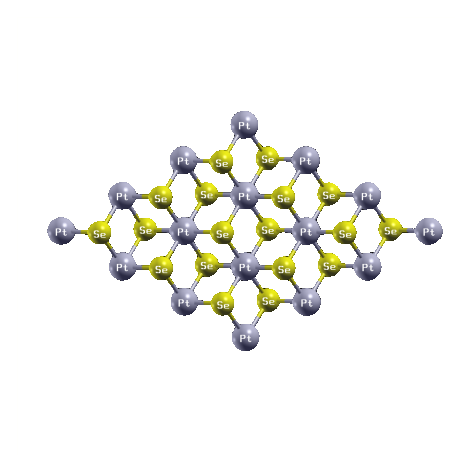
\epsfig{file=figRes/PtSe2/est/est1.eps, width=6cm, height=6cm}
		\label{Sim:fig:estptse2arr}
	}
    \subfigure[vista de lado]{
    	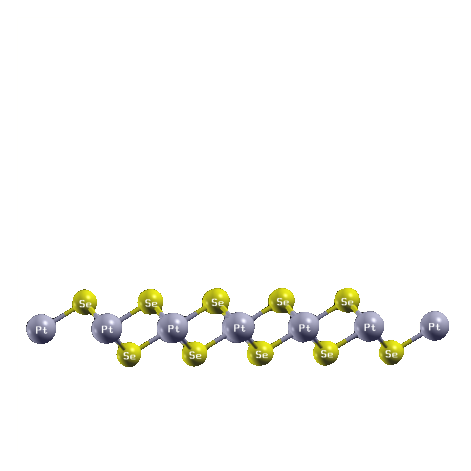
\epsfig{file=figRes/PtSe2/est/est2.eps, width=6cm, height=6cm}
    	\label{Sim:fig:estptse2lado}
    }
   \caption[Vista de la supercelda de PtSe\textsubscript{2}.]{Vista de la estructura de $PtSe_2$ en la que se repiten 3 veces la celda unitaria en dos direcciones.}
   \label{Sim:fig:estptse2}
\end{figure}
\newline
En la figura \ref{Sim:fig:bandasptse2} se muestra el diagrama de bandas con acople spin-\'orbita (fig \ref{Sim:fig:bandSocptse2}) y sin este  efecto (fig. \ref{Sim:fig:bandnoSocptse2}). La principal caracter\'istica de este material es que en el caso de una mono-capa es un semiconductor indirecto, encontr\'andose el m\'inimo de la banda de conducci\'on entre los puntos $\Gamma$ y $M$ y el m\'aximo de la banda de valencia se encuentra entre el punto $M$ y $\Gamma$ (~$0.20 \AA^{-1}$ del punto $\Gamma$); desplazándose  al punto $\Gamma$ cuando se incluye el efecto de spin-\'orbita, debido a que  las bandas que son degeneradas en el punto $\Gamma$  en la banda de valencia,  se separan $\Delta_{so}^{v,\Gamma}=333.41 ~meV$ y en el punto $K$ se distancian $\Delta_{so}^{v,K}=163 ~meV$. Adem\'as  se observa que la separaci\'on entre las dos primeras bandas de conducci\'on de $\Delta_{so}^{c,\Gamma} = 57.48~ meV$ en el punto $\Gamma$ y de $\Delta_{so}^{c,K} = 2.1 ~meV$ en el punto $K$, los cuales son mas peque\~nos que en la banda de valencia. Estos rompimientos de la degeneraci\'on provocan que el tama\~no de la brecha prohibida se reduzca a $1.2 ~eV$. Si se observa la densidad de estados, se puede notar que la banda de valencia est\'a formada principalmente por los electrones de  orbitales $d$ del Platino, con excepci\'on  del m\'aximo de la banda de valencia el cual est\'a formado mayoritariamente por los orbitales $p$ del Selenio, con una mezcla de orbitales $d$ del Platino. En el caso de la banda de conducci\'on, la contribuci\'on de ambos orbitales es casi la misma y su distribuci\'on en el diagrama de bandas se observa en la figura \ref{Sim:fig:pdosPtse2cU}, la cual est\'a formada por el mapeo de la densidad de estados proyectada sobre el respectivo orbital en la primera zona de Brillouin.

\begin{figure}[!hbt]
	\centering
	\subfigure[con acople spin-\'orbita]{
		\includegraphics[scale=1]{figRes/PtSe2/bandas/bandasDOS.pdf}
		\label{Sim:fig:bandSocptse2}
	}
    \subfigure[sin acople spin-\'orbita]{
    	\includegraphics[scale=1]{figRes/PtSe2/bandas/noSOC/bandasDOSnoSoc.pdf}
    	\label{Sim:fig:bandnoSocptse2}
    }
\caption[Diagrama de bandas y densidad de estados de la celda unitaria del PtSe\textsubscript{2}.]{Gr\'aficas del diagrama de bandas y la densidad de estados del PtSe\textsubscript{2} (\ref{Sim:fig:bandSocptse2}) incluyendo el acople spin-\'orbita y (\ref{Sim:fig:bandnoSocptse2}) sin este efecto.}
\label{Sim:fig:bandasptse2}
\end{figure}



 Dado que la magnetizaci\'on es cero, se puede decir que el material es no-magn\'etico incluso si se incluye el efecto de spin-\'orbita. Esto se puede explicar debido a que el Platino, que  tiene seis electrones del orbital $d$  $(Pt^{4+})$ se encuentran de forma estable en el estado $t_{2g}$ \cite{doi:10.1063/1.4955468} y por lo tanto, no cuentan con   un orden magn\'etico entre los \'atomos de Platino. 
\begin{figure}[!hbt]
	\centering
	\includegraphics[scale=1]{figRes/PtSe2/bandas/projbandorb/orbproj.pdf}
	\caption[Distribuci\'on de orbitales $d$ y $p$ del Platino y Selenio respectivamente el ep PtSe\textsubscript{2}.]{Distribuci\'on de los orbitales $d$ del platino y $p$ del Selenio en el PtSe\textsubscript{2} sin el efecto de spin-\'orbita y considerando una densidad de estados mayor a 0.1 estados/eV. }
	\label{Sim:fig:pdosPtse2cU}
\end{figure}
\subsection{PtS\textsubscript{2}} \label{Sim:subsec:pts2celu}
Un material muy similar  es el Disulfuro de Platino el cual cuenta con la misma estructura que el di seleniuro de platino. En la tabla \ref{Sim:tabla:pts2est} se muestra la comparaci\'on con los datos experimentales y de otras simulaciones con los obtenidos en este trabajo y se puede observar que estos resultados son muy similares a los reportados de simulaciones y de par\'ametros experimentales. En el caso de la brecha prohibida se obtiene tambi\'en un valor parecido al obtenido experimentalmente. Se puede notar que en comparaci\'on con los datos correspondientes al PtSe\textsubscript{2}, el PtS\textsubscript{2} tiene una constante de red mas peque\~na as\'i como los dem\'as par\'ametros estructurales. En cambio el tama\~no de la brecha prohibida es mayor en el PtS\textsubscript{2}, lo cual podr\'ia indicar que las interacciones entre los \'atomos de Azufre y Platino es mayor que el caso del Platino y Selenio.
\begin{table}
	\centering
	\caption[Comparaci\'on de par\'ametros estructurales del PtS\textsubscript{2}.]{Se comparan los mismos par\'ametros que en el cuadro \ref{Sim:tabla:ptse2est} pero se cambia el \'atomo de Selenio por uno de azufre }
	\begin{tabular}{|c|c|c|c|c|c|}
		\hline
		& $a_0~(\AA)$   & $d_{Pt-S}~(\AA)$  & $d_{S-S}~(\AA)$  &  $\theta_{S-Pt-S}~(grado)$ & $E_g~(eV)$ \\
		\hline
		\hline
		calc.   & $3.5785$& $2.4072 $     & $3.2207 $  & $96.04$              & $1.3911 ~(1.724)$\\
		ref. \cite{doi:10.1021/jp405808a,DU201}    & $3.57$& $2.40 $     & $3.21 $  & $96.18$              & $1.81 ~(1.76)$\\
		exp. \cite{datexpPt,https://doi.org/10.1002/adma.201504572}   & $3.5432$& $2.34 $     & $3.07 $  & $98.21$              & $1.6$\\
		\hline
		
	\end{tabular}
	\label{Sim:tabla:pts2est}
\end{table}
%\newline
\newline
\par En la figura \ref{Sim:fig:bandaspts2} se muestra la estructura de bandas del PtS\textsubscript{2} con efectos de acople spin-\'orbita (fig. \ref{Sim:fig:bandSocpts2}) y sin este (fig. \ref{Sim:fig:bandnoSocpts2}). Se puede notar que este material es un semiconductor indirecto con el m\'inimo de la banda de conducci\'on que se encuentra entre el punto $\Gamma$ y $M$ al igual que con el PtS\textsubscript{2}. Pero en el caso de la banda de valencia no sucede lo mismo ya que cuando se incluyen los efectos de spin \'orbita, el m\'aximo de la banda de valencia no se encuentra en el punto $\Gamma$ sino que se localiza entre el punto $\Gamma$ y $K$ a $0.23 \AA^{-1}$ del punto $\Gamma$. En cuanto al rompimiento de la degeneraci\'on por el efecto de spin-\'orbita, se observa una separaci\'on entre las bandas del m\'aximo de la banda de valencia en el punto $\Gamma$ que es $\Delta_{so}^{v,\Gamma}= 207.1~ meV$ y en el punto $K$ es de $\Delta_{so}^{v,K}= 195~ meV$. Para el caso de  la separaci\'on entre las dos  primeras bandas de conducci\'on  en el punto $\Gamma$ es de $\Delta_{so}^{c,\Gamma}= 256~ meV$ y en el punto $K$ es de  $\Delta_{so}^{v,K}= 107~ meV$. Comparando estos valores con los obtenidos para el PtSe\textsubscript{2} se observa que, a excepci\'on del punto $\Gamma$ en la banda de valencia,  son mayores las separaciones $\Delta_{so}$ en el PtS\textsubscript{2}, debido  a que a diferencia del PtSe\textsubscript{2} no sucede una disminuci\'on tan marcada de los estados correspondientes a los orbitales $d$ del Platino cerca del m\'aximo de la banda de valencia.  En la banda de conducci\'on es ligeramente  mayor la poblaci\'on de estos electrones $d$ que la de los electrones del orbital $p$ del Selenio. En la figura \ref{Sim:fig:pdosPts2cU} se muestra la distribuci\'on de los estados de dichos dos orbitales en el diagrama de bandas, en el que se puede notar que los electrones $d$ del platino se encuentran mas distribuidos en el m\'aximo de la banda de valencia en comparaci\'on del PtSe\textsubscript{2}. El efecto de spin-\'orbita provoca que el tama\~no de la brecha prohibida se reduzca a $1.72~ eV$ el cual es un valor cercano al medido experimentalmente\cite{https://doi.org/10.1002/adma.201504572}.
\newline
En el caso del c\'alculo de la magnetizaci\'on, se encontr\'o que es $0 ~\mu_{B}/celda$, el cual es el mismo resultado que se obtuvo para el PtSe\textsubscript{2} y el motivo de que \'este material no sea magn\'etico es el mismo que para el PtSe\textsubscript{2}.
\begin{figure}[!hbt]
	\centering
	\subfigure[con acople spin-\'orbita]{
		\includegraphics[scale=1]{figRes/PtS2/bandas/celu/soc/bandasDOS.pdf}
		\label{Sim:fig:bandSocpts2}
	}
	\subfigure[sin acople spin-\'orbita]{
		\includegraphics[scale=1]{figRes/PtS2/bandas/celu/nosoc/bandasDOSnoSoc.pdf}
		\label{Sim:fig:bandnoSocpts2}
	}
	\caption[Diagrama de bandas y densidad de estados de la celda unitaria del PtS\textsubscript{2}.]{Gr\'aficas del diagrama de bandas y la densidad de estados del PtS\textsubscript{2} (\ref{Sim:fig:bandSocpts2}) incluyendo el acople spin-\'orbita y (\ref{Sim:fig:bandnoSocpts2}) sin este efecto.}
	\label{Sim:fig:bandaspts2}
\end{figure}
\begin{figure}[!hbt]
	\centering
	\includegraphics[scale=1]{figRes/PtS2/bandas/celu/projbandas/orbproj.pdf}
	\caption[Distribuci\'on de orbitales $d$ y $p$ del Platino y Selenio respectivamente el ep PtS\textsubscript{2}.]{Distribuci\'on de los orbitales $d$ del platino y $p$ del Selenio en el PtS\textsubscript{2} sin el efecto de spin-\'orbita y considerando una densidad de estados mayor a 0.1 estados/eV. }
	\label{Sim:fig:pdosPts2cU}
\end{figure}

\begin{table}
	\centering
	\caption[Comparaci\'on de par\'ametros estructurales del VSe\textsubscript{2}.]{Se comparan los mismos par\'ametros que en el cuadro \ref{Sim:tabla:ptse2est} pero se cambia el \'atomo de Platino por uno de Vanadio  y sin considerar el tama\~no de la brecha prohibida}
	\begin{tabular}{|c|c|c|c|c|}
		\hline
		& $a_0~(\AA)$   & $d_{V-Se}~(\AA)$  & $d_{Se-Se}~(\AA)$  &  $\theta_{Se-V-Se}~(grado)$ \\
		\hline
		\hline
		calc.   & $3.3403$& $2.4924 $     & $3.7 $  & $84.15$ \\
		ref. \cite{doi:10.1021/jp405808a}    & $3.32$& $2.48 $     & $3.7 $  & $83.81$ \\
		exp. \cite{expVse}   & $3.355$& $2.47 $     & $3.627 $  & $85.53$\\
		\hline
		
	\end{tabular}
	\label{Sim:tabla:VSe2est}
\end{table}
\subsection{VSe\textsubscript{2}} \label{Sim:subsec:vse2cU}
Los resultados estructurales y su comparaci\'on con otros trabajos se muestran en la tabla \ref{Sim:tabla:VSe2est}, se puede observar que los valores obtenidos son menores a los dos materiales analizados anteriormente, aunque se sigue manteniendo la estructura 1T estable. En este no existe una brecha prohibida  lo que indica que este material  se comporta como un metal. En la figura \ref{Sim:fig:bandasVSe2} se observan el diagrama de bandas con el efecto de spin-\'orbita(fig. \ref{Sim:fig:bandSocVSe2}) y sin este (fig \ref{Sim:fig:bandnoSocVse2}). En dicha situación  se muestran las bandas orientadas con el spin ($1/2,~ \uparrow$) y con el spin ($-1/2,~ \downarrow$) y es posible observar que el n\'umero de estados no es el mismo para estas dos componentes,  provocando una magnetizaci\'on de $0.62~ \mu_B / celda$.
\begin{figure}[!hbt]
	\centering
	\subfigure[con acople spin-\'orbita]{
		\includegraphics[scale=1]{figRes/VSe2/bandas/celU/soc/bandasDOS.pdf}
		\label{Sim:fig:bandSocVSe2}
	}
	\subfigure[sin acople spin-\'orbita]{
		\includegraphics[scale=0.9]{figRes/VSe2/bandas/celU/nosoc/bandasDOSnoSoc.pdf}
		\label{Sim:fig:bandnoSocVse2}
	}
	\caption[Diagrama de bandas y densidad de estados de la celda unitaria del VSe\textsubscript{2}.]{Gr\'aficas del diagrama de bandas y la densidad de estados del VSe\textsubscript{2} (\ref{Sim:fig:bandSocVSe2}) incluyendo el acople spin-\'orbita y (\ref{Sim:fig:bandnoSocVse2}) sin este efecto.}
	\label{Sim:fig:bandasVSe2}
\end{figure}
\newline
Si se observa la figura \ref{Sim:fig:bandSocVSe2} se nota que las separaciones que induce el efecto de spin- \'orbita el las bandas por debajo del nivel de Fermi  son muy peque\~nas en los puntos $\Gamma$, $M$ y $K$, aunque estas aumentan el las posiciones intermedias entre estos, lo cual   permite separar las bandas degeneradas que corresponden a distintos spines (fig \ref{Sim:fig:bandnoSocVse2}). adem\'as, se puede observar en la densidad de estados que estas bandas est\'an compuestas por los electrones en el orbital $p$ de Selenio mezclados con electrones del orbital $d$ del vanadio a diferencia de   los estados cercanos y superiores al nivel de Fermi  que est\'an compuestos por los electrones del orbital $d$ del Vanadio, principalmente. Tal y como se muestra en la densidad de estados (fig. \ref{Sim:fig:bandnoSocVse2}) los orbitales $d$ de Vanadio contribuyen  considerablemente a la aparici\'on del momento magn\'etico distinto de cero. En la figura \ref{Sim:fig:pDOSvVse2} se aprecia que la mayor contribuci\'on a los estados ocupados cercanos al nivel de Fermi, proviene del orbital $d_{z^2}$ y en los estados mas lejanos por los orbitales $d_{zx}$ y $d_{zy}$; por lo que se espera que los electrones de los estados ocupados tengan el spin orientado en la direcci\'on perpendicular al plano de la muestra. Los estados no ocupados esencialmente est\'an formados por los orbitales $d_{x^2 -y^2}$ y $d_{xy}$, en donde los \'atomos de vanadio aportan una magnetizaci\'on de $0.61~ \mu_{B}$.   
\begin{figure}[!hbt]
	\centering
	\includegraphics[scale=1]{figRes/VSe2/bandas/celU/nosoc/pdosV.pdf}
	\caption[Densidad de estados proyectada de los orbitales $d$ del vanadio en VSe\textsubscript{2}.]{densidad de estados parcial de los orbitales $d$ del \'atomo de Vanadio en VSe\textsubscript{2}, la flecha azul y roja indican la densidad de estados de los spines $1/2$ y $-1/2$ respectivamente.}
	\label{Sim:fig:pDOSvVse2}
\end{figure}
\newline
En la figura \ref{Sim:fig:pDOSseVse2} se observa la densidad de estados proyectada en los orbitales $p$ del \'atomo de Selenio, se puede observar que los orbitales $p_{x}$ son los que contribuyen a los estados en el VSe\textsubscript{2}, as\'i mimo se nota que los \'atomos de selenio aportan una magnetizaci\'on de $ -0.038~ \mu_{B}$.
\begin{figure}[!hbt]
	\centering
	\includegraphics[scale=1]{figRes/VSe2/bandas/celU/nosoc/pdosSe.pdf}
	\caption[Densidad de estados proyectada de los orbitales $p$ del Selenio en VSe\textsubscript{2}.]{densidad de estados parcial de los orbitales $p$ del \'atomo de Selenio en VSe\textsubscript{2}, la flecha azul y roja indican la densidad de estados de los spines $1/2$ y $-1/2$ respectivamente.}
	\label{Sim:fig:pDOSseVse2}
\end{figure}
%\newline
\par En la figura \ref{Sim:fig:distmagnVse2} se muestra la distribuci\'on de spines  y se puede notar que en los \'atomos de Vanadio se concentran los  valores positivos para el spin y en los \'atomos de Selenio se concentra una peque\~na contribuci\'on negativa que, de acuerdo a la densidad de estados, esta proviene de el orbital $p_x$; as\'i mismo, se observa una peque\~na contribuci\'on positiva que se puede atribuir a los orbitales $p_z$.
\begin{figure}[!hbt]
	\centering
	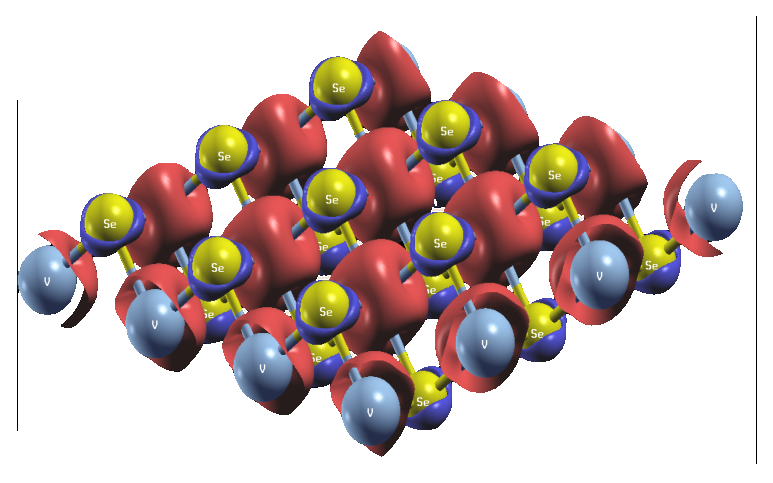
\epsfig{file=figRes/VSe2/vse2magz.eps, scale=0.65}
	\caption[Distribuci\'on de spin en VSe\textsubscript{2}]{Distribuci\'on  de spin en el VSe\textsubscript{2} visualizada con XcrySDen, en donde se muestra un valor de iso superficie de $\pm 0.002$, en donde el color rojo indica un valor positivo y el azul el negativo.}
	\label{Sim:fig:distmagnVse2}
\end{figure}
\subsection{VS\textsubscript{2}} \label{Sim:subsec:VS2}
Este material en la estructura 1T tiene características muy similares al VSe\textsubscript{2}, en la tabla \ref{Sim:tabla:VS2est} se muestran los par\'ametros estructurales calculados en este trabajo y su comparaci\'on con otras simulaciones. Para este material no existen muchos estudios experimentales y es por esta raz\'on  que solamente se muestra el tama\~no de red, el cual es muy cercano al calculado. De igual forma los par\'ametros calculados en este trabajo son muy parecidos a  otras simulaciones realizadas anteriormente.
%\newline

\begin{table}
	\centering
	\caption[Comparaci\'on de par\'ametros estructurales del VS\textsubscript{2}.]{Par\'ametros estructurales para el VS\textsubscript{2} y su comparaci\'on con otras simulaciones y con datos obtenidos por experimentos.}
\begin{tabular}{|c|c|c|c|c|}
	\hline
	& $a_0~(\AA)$   & $d_{V-S}~(\AA)$  & $d_{S-S}~(\AA)$  &  $\theta_{S-V-S}~(grado)$ \\
	\hline
	\hline
	calc.   & $3.1939$& $2.3556 $     & $3.4632 $  & $85.367$ \\
	ref. \cite{doi:10.1021/jp405808a}    & $3.17$& $2.35 $     & $3.46 $  & $85.04$ \\
	exp. \cite{C9QI01142K}   & $3.22$& $-- $     & $-- $  & $--$\\
	\hline
	
\end{tabular}
\label{Sim:tabla:VS2est}
\end{table}

\par En la figura \ref{Sim:fig:bandasVS2} se muestra el diagrama de bandas  con el efecto de spin-\'orbita(fig. \ref{Sim:fig:bandSocVS2}) y sin este fig. (\ref{Sim:fig:bandnoSocVs2}). En el caso en el que considera el acople spin-\'orbita se observa el mismo fen\'omeno que en el caso del VSe\textsubscript{2}, es decir en los puntos de alta simetr\'ia ($\Gamma$, $K$ y $M$) el rompimiento de la degeneraci\'on en las bandas con distinto spin (se pueden observar en la Fig. \ref{Sim:fig:bandnoSocVs2}) es muy peque\~no y en las posiciones intermedias entre estos puntos aumenta la separaci\'on entre estas bandas,  permitiendo diferenciar entre bandas de distinto spin. En el caso de los estados por encima del nivel de Fermi, se tienen un conjunto bien determinado por bandas orientadas con spin $\uparrow$ y otras con spin $\downarrow$ y est\'an formadas principalmente por el orbital $d$ del Vanadio. En general se observa que la separaci\'on entre las bandas son peque\~nas debido a que el \'atomo de Vanadio no es muy pesado en comparaci\'on con el Platino.
\newline %\newline
\par En el caso del c\'alculo de la magnetizaci\'on se encontr\'o que este material es ferromagn\'etico debido a que la magnetizaci\'on tiene un valor de $0.55 ~\mu_{B}/celda$, el cual es un valor menor a que se obtuvo en el caso de VSe\textsubscript{2}. Observando la densidad de estados en la figura \ref{Sim:fig:bandnoSocVs2} se nota que en los estados por debajo del nivel de Fermi, el orbital $d$ del \'atomo de vanadio esta un poco delocalizado y  la poblaci\'on de los orbitales $p$ del \'atomo de Azufre es muy similar al del vanadio, lo cual podr\'ia sugerir que estos orbitales se hibridizan  y forman enlaces covalentes entre estos dos \'atomos y este es un fen\'omeno que tambi\'en se observa en el los materiales descritos anteriormente.
\begin{figure}[!hbt]
	\centering
	\subfigure[con acople spin-\'orbita]{
		\includegraphics[scale=1]{figRes/VSe2/bandas/celU/soc/bandasDOS.pdf}
		\label{Sim:fig:bandSocVS2}
	}
	\subfigure[sin acople spin-\'orbita]{
		\includegraphics[scale=0.9]{figRes/VS2/celdaU/estructura electronica/noSOC/bandasDOSnoSoc.pdf}
		\label{Sim:fig:bandnoSocVs2}
	}
	\caption[Diagrama de bandas y densidad de estados de la celda unitaria del VS\textsubscript{2}.]{Gr\'aficas del diagrama de bandas y la densidad de estados del VS\textsubscript{2} (\ref{Sim:fig:bandSocVS2}) incluyendo el acople spin-\'orbita y (\ref{Sim:fig:bandnoSocVs2}) sin este efecto.}
	\label{Sim:fig:bandasVS2}
\end{figure}
\newline

\par Estudiando los orbitales $d$ del \'atomo de vanadio (fig. \ref{Sim:fig:pDOSvVs2}) se observa que, al igual que en el caso del VSe\textsubscript{2},  el orbital $d_{z^2}$ es el que tiene la mayor contribución a los  estados por debajo del nivel de Fermi y que por lo general se encuentran delocalizados. Para los estados  desocupados estos est\'an formados por orbitales $d_{x^2-y^2}$ y $d_{xy}$, los cuales est\'an muy localizados. Dichos orbitales tambi\'en tienen importantes contribuciones en los estados que se encuentran ocupados, los orbitales $d_{zx}$ y $d_{zy}$ tienen contribuciones importantes en los estados m\'as cercanos al n\'ucleo y si se toma en consideraci\'on que los estados orientados en la direcci\'on $z$, se espera que los spines est\'en orientados en esa direcci\'on. La magnetizaci\'on que aporta el \'atomo de Vanadio es de $ 0.5 ~\mu_{B} $.
\begin{figure}[!hbt]
	\centering
	\includegraphics[scale=1]{figRes/VSe2/bandas/celU/nosoc/pdosV.pdf}
	\caption[Densidad de estados proyectada de los orbitales $d$ del Vanadio en el VS\textsubscript{2}.]{Densidad de estados parcial de los orbitales $d$ del \'atomo de Vanadio en VSe\textsubscript{2}, la flecha azul y roja indican la densidad de estados de los spines $1/2$ y $-1/2$ respectivamente.}
	\label{Sim:fig:pDOSvVs2}
\end{figure}
%\newline
En el caso de los orbitales $p$ de \'atomo del Azufre (fig. \ref{Sim:fig:pDOSsVs2}) se puede observar que la mayor contribuci\'on proviene del  orbital $p_x$ y es el que participa con los enlaces covalentes con el Vanadio. Los \'atomos de Azufre contribuyen con una magnetizaci\'on de $-0.024 ~\mu_{B} $. 
%\newline
\newline

\begin{figure}[!hbt]
	\centering
	\includegraphics[scale=1]{figRes/VS2/celdaU/estructura electronica/noSOC/pdosS.pdf}
	\caption[Densidad de estados proyectada de los orbitales $p$ del Azufre en el VS\textsubscript{2}.]{Densidad de estados parcial de los orbitales $p$ del \'atomo de Azufre en VS\textsubscript{2}, la flecha azul y roja indican la densidad de estados de los spines $1/2$ y $-1/2$ respectivamente.}
	\label{Sim:fig:pDOSsVs2}
\end{figure}
\par En la figura \ref{Sim:fig:distmagnVs2} se muestra la distribuci\'on de spines  y se puede notar, al igual que en el caso del VSe\textsubscript{2}, que en los \'atomos de Vanadio se concentran los  valores positivos para el spin y en los \'atomos de Azufre se concentra una peque\~na contribuci\'on negativa que, de acuerdo a la densidad de estados, esta proviene de el orbital $p_x$; as\'i mismo, se observa una peque\~na contribuci\'on positiva que se puede atribuir a los orbitales $p_z$.

 \begin{figure}[!hbt]
 	\centering
 	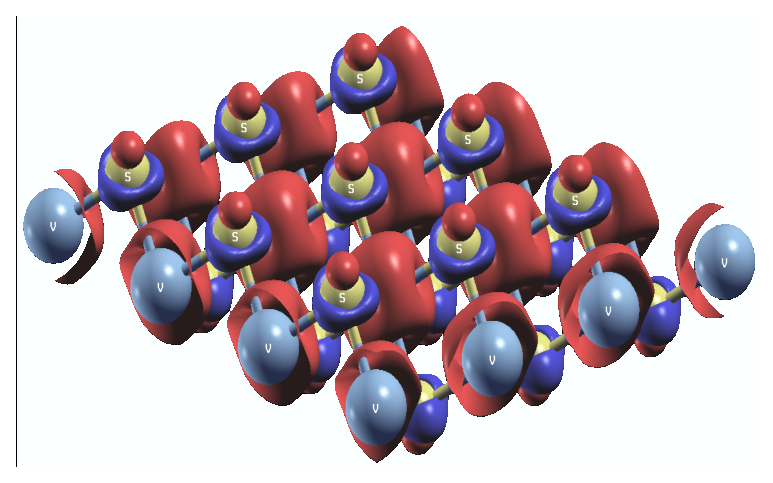
\epsfig{file=figRes/VS2/vs2magz.eps, scale=0.65}
 	\caption[Densidad de spin en el VS\textsubscript{2}.]{Distribuci\'on  de spin en el VS\textsubscript{2} en donde se muestra un valor de iso superficie de $\pm 0.002$, en donde el color rojo indica un valor positivo y el azul el negativo.}
 	\label{Sim:fig:distmagnVs2}
 \end{figure}
\section{An\'alisis de la introducci\'on de una vacancia de metal de transición } \label{Sim:sec:MdefVac}
A continuaci\'on se explica el comportamiento de la magnetizaci\'on por la introducci\'on de una vacancia del metal de transición en los materiales descritos anteriormente. El la sub secci\'on \ref{Sim:subsec:vacPt} se explica el efecto de la vacancia de Platino en PtSe\textsubscript{2} y PtS\textsubscript{2} y en la subsecci\'on \ref{Sim:subsec:vacV} se estudia el efecto de la vacancia de Vanadio en el VSe\textsubscript{2} y VS\textsubscript{2}.
\subsection{Vacancia de Platino en PtSe\textsubscript{2} y PtS\textsubscript{2}} \label{Sim:subsec:vacPt}
En la figura \ref{Sim:fig:supVac} se muestran las superceldas con la vacancia de platino en PtSe\textsubscript{2} y PtS\textsubscript{2}; se nota que los \'atomos de Selenio o Azufre que son vecinos al \'atomo faltante, indicado con lineas punteadas azules, se alejan entre si acerc\'andose a los \'atomos de Platino  vecinos. Este fen\'omeno debe a que los electrones que formaban parte de los enlaces covalentes con el \'atomo de platino quedan libres y aparece une gas de electrones en el lugar de la  vacancia. Para poder apreciar este efecto se muestra en la figura \ref{Sim:fig:cargavac}  la distribuci\'on de carga para valores positivos en escala logar\'itmica para las supercelda de PtSe\textsubscript{2} y  PtS\textsubscript{2}, se puede observar que existe una peque\~na distribuci\'on de electrones en el lugar del \'atomo faltante.

\begin{figure}[!hbt]
	\centering
	\subfigure[en PtSe\textsubscript{2}]{
		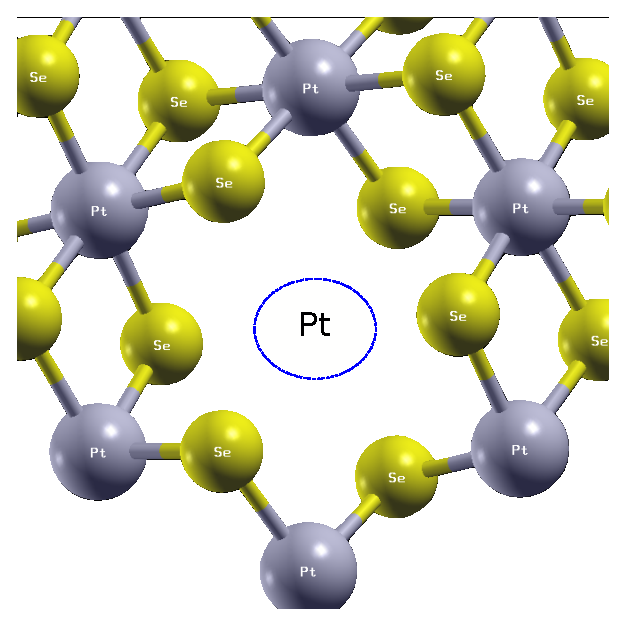
\epsfig{file=figRes/PtSe2/VacanciaPt.eps, scale=0.6}
	\label{Sim:fig:supVacptse2}
	}
    \subfigure[en PtS\textsubscript{2}]{
    	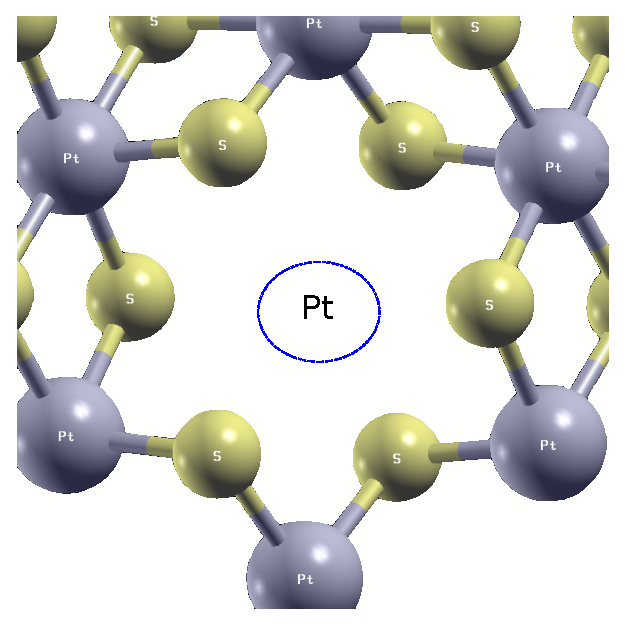
\epsfig{file=figRes/PtS2/VacanciaPt.eps, scale=0.6}
    	\label{Sim:fig:supVacpts2}
    }
    \caption[Superceldas de  PtSe\textsubscript{2} y PtS\textsubscript{2} con vacancia de Platino.]{Supercelda con vacancia de Platino en PtSe\textsubscript{2} (\ref{Sim:fig:supVacptse2}) y PtS\textsubscript{2} (\ref{Sim:fig:supVacpts2}).}
    \label{Sim:fig:supVac}
\end{figure}

\begin{figure}[!hbt]
	\centering
	\subfigure[PtSe\textsubscript{2}]{
		\includegraphics[scale=0.8]{figRes/PtSe2/densidades/densPos/densidadpos.pdf}
		\label{Sim:fig:cargavacPtse2}
	}
   \subfigure[PtS\textsubscript{2}]{
   	\includegraphics[scale=0.8]{figRes/PtS2/def/densidades/denspos/densidadpos.pdf}
   	\label{Sim:fig:cargavacPts2}
   }
  \caption[Distribuci\'on de carga en alrededor de la vacancia de platino en PtSe\textsubscript{2} y PtSe\textsubscript{2}.]{Distribuci\'on de carga alrededor de la vacancia de platino en PtSe\textsubscript{2} (\ref{Sim:fig:cargavacPtse2}), y en PtS\textsubscript{2} (\ref{Sim:fig:cargavacPtse2}).}
 \label{Sim:fig:cargavac}	
\end{figure}
%\newline
%\newline
En la figura \ref{Sim:fig:bandasSOCPtSe2vac} se muestra el diagrama de bandas con su densidad de estados,donde  se puede apreciar que el principal efecto que se observa es la aparici\'on de  dos niveles dentro de la banda prohibida y al aumento de la separaci\'on entre los dos \'ultimos niveles de la banda de valencia. Adicionalmente se puede notar que en la densidad de estados, los dos niveles dentro de la brecha prohibida provienen de los orbitales $p$ del \'atomo de Selenio vecino a la vacancia; mientras que el orbital $p$ de un \'atomo de selenio, que mantiene sus enlaces originales completos, no contribuye considerablemente a la creación de estos niveles. en relaci\'on a los orbitales $d$ del platino,  la casi igualdad que exist\'ia con los orbitales $p$ del Selenio en la banda de conducci\'on desaparece y ahora la mayor contribuci\'on viene de los orbitales de Selenio que no son vecinos de la vacancia.

\begin{figure}
	\centering
	\includegraphics[width=12cm, height=7cm]{figRes/PtSe2/def/bandas/comparacionbandas/bandasDOS.pdf}
	\caption[Diagrama de bandas y densidad de estados del PtSe\textsubscript{2} con vacancia de Platino y efecto spin-\'orbita.]{diagrama de bandas y la densidad de estados mostrando las contribuciones del orbital $d$ del Platino y $d$ del \'atomo de Selenio vecino del \'atomo faltante y otro que no lo es.}
	\label{Sim:fig:bandasSOCPtSe2vac}
\end{figure}

Mediante la introducci\'on de este defecto se observa que aparece un momento magn\'etico de $2.37~ \mu_{B}/celda$. En la figura \ref{Sim:fig:bandDefPtse2noSOC} se muestra el diagrama de bandas sin el efecto de spin-\'orbita y se puede observar que  las bandas con spin $\uparrow$ y $\downarrow$ se encuentran bien distribuidas y separadas;  adem\'as se tiene que las  bandas inducidas por efecto de la vacancia  dentro de la brecha prohibida   corresponden principalmente al  spin $\downarrow$  y de acuerdo  a la densidad de estados que se muestra a la izquierda del diagrama de bandas, \'estas est\'an formadas principalmente por electrones en el orbital $p$ de los \'atomos vecinos a la vacancia de Platino, sugiriendo   que estas  provienen de los electrones que quedan libres por los enlaces covalentes rotos. Adem\'as  se reporta la densidad de estados del orbital $p$ de un \'atomo de Selenio que no se ve afectado directamente por la vacancia,  donde que su distribuci\'on es muy similar a la observada en un material sin defectos, de tal forma que aporta una magnetizaci\'on de $0.003 ~\mu_{B}$.

\begin{figure}[!hbt]
	\centering
	\includegraphics[scale=0.9]{figRes/PtSe2/def/bandas/nosoc/bandasDOSnoSoc.pdf}
	\caption[Diagrama de bandas y densidad de estados del PtSe\textsubscript{2} con vacancia de Platino.]{Diagrama de bandas y densidad de estados sin incluir el efecto de spin \'orbita en el PtSe\textsubscript{2}, se muestran las bandas correspondientes a cada spin y en el caso de la densidad de estados se muestra las contribuciones del orbital $d$ del Platino y el $p$ del \'atomo de Selenio vecino de la vacancia y de un \'atomo que a\'un mantiene los tres enlaces covalentes.}
	\label{Sim:fig:bandDefPtse2noSOC}
\end{figure}

\begin{figure}[!hbt]
	\centering
	\includegraphics[scale=0.9]{figRes/PtSe2/def/bandas/nosoc/pdosS_neg.pdf}
	\caption[Densidad de estados proyectado en el orbital $p$ del \'atomo de Selenio en el PtSe\textsubscript{2} con vacancia de Platino.]{Densidad de estados del orbital $p$ del \'atomo de Selenio vecino de la vacancia de platino.}
	\label{Sim:fig:pdosSeptse2vac}
\end{figure} 

Para el orbital $p$ del \'atomo vecino a la vacancia de Platino,  se puede  observar en la figura \ref{Sim:fig:pdosSeptse2vac} que los estados generados dentro de la brecha prohibida provienen mayoritariamente de  los orbitales $p_z$ y $p_y$. Adem\'as, por debajo del nivel de Fermi (representado cono una l\'inea punteada en la figura \ref{Sim:fig:pdosSeptse2vac}) se puede observar que la diferencia en el n\'umero de estados con spin $\uparrow$ y $\downarrow$ para las tres componentes del orbital $p$ y la diferencia es mayor para los orbitales $p_x$ y $p_y$, por lo que se espera que el spin est\'e orientado en la direcci\'on del plano del sistema. Se tiene entonces un total una contribuci\'on al momento magn\'etico  de $0.224 ~\mu_{B}$. Para  la densidad de estados del orbital $d$ del Platino,  se  nota que la mayor contribuci\'on al momento magn\'etico proviene de los orbitales $d_{x^2-y^2}$ y $d_{xy}$ que est\'an orientados en la direcci\'on del plano del sistema y que tambi\'en presenta una contribuci\'on mas peque\~na de los orbitales $d_{zx}$ y $d_{zy}$, principalmente formando los estados de la banda de conducci\'on y en total el \'atomo de platino contribuye  con un momento magn\'etico de $0.03~ \mu_{B}$.

\begin{figure}[!hbt]
	\centering
	\includegraphics[scale=1]{figRes/PtSe2/def/bandas/nosoc/pdosPt_3.pdf}
	\caption[Densidad de estados proyectado del orbital $d$ del Platino en el PtSe\textsubscript{2} con vacancia de Platino.]{Densidad de estados del orbital $d$ del \'atomo de Platino.}
	\label{Sim:fig:pdosPtdtse2vac}
\end{figure}  
\par En el caso del PtS\textsubscript{2} se observan en la figura \ref{Sim:fig:VacPtsocPtS2} el diagrama de bandas con el efecto de spin-\'orbita y la densidad de estados con  el pDOS del orbital $d$ del \'atomo de Platino y el orbital $p$ de un \'atomo de Azufre vecino a la vacancia y  de uno que no lo es. Se observa que aparecen algunas bandas dentro de la brecha prohibida y las cuales son muy similares a las observadas en el PtSe\textsubscript{2}, aunque se observa que el nivel de Fermi se desplaza dentro de la banda de valencia y se ve que los estados dentro de la brecha prohibida provienen de los \'atomos de Azufre vecinos a la vacancia.
\begin{figure}[!hbt]
	\centering
	\includegraphics[width=12cm, height=7cm]{figRes/PtS2/def/bandas/soc/bandasDOS.pdf}
	\caption[Diagrama de bandas y densidad de estados incluyendo el efecto de spin-\'orbita en PtS\textsubscript{2} con una vacancia de Platino]{Diagrama de bandas y densidad de estados del PtS\textsubscript{2} con vacancia de Platino incluyendo el efecto de spin-\'orbita.}
	\label{Sim:fig:VacPtsocPtS2}
\end{figure}

En este caso aparece un momento magn\'etico de $2.63 ~ \mu_{B}/celda$. En la figura \ref{Sim:fig:noSOCpts2def} se muestra el diagrama de bandas indicando su distribuci\'on  para cada spin $\uparrow$ y $\downarrow$. N\'otese que las bandas que se generan por el efecto de la vacancia provienen del orbital $p$ del \'atomo de Azufre, cercano a la vacancia del Platino. De igual manera que con el PtSe\textsubscript{2} el \'atomo de Azufre que no se ve afectado por la vacancia, no muestra una magnetizaci\'on considerable; adem\'as de que la densidad de estados correspondiente al orbital $p$ de este \'atomo no es muy distinta al del sistema sin deformar.
\newline

\begin{figure}[!hbt]
	\centering
	\includegraphics[scale=0.9]{figRes/PtS2/def/bandas/nosoc/bandasDOSnoSoc.pdf}
	\caption[Diagrama de bandas y densidad de estados del PtS\textsubscript{2} con una vacancia de Platino.]{Diagrama de bandas y densidad de estados del PtS\textsubscript{2} en donde se muestra la distribuci\'on del spin, en el caso de la densidad de estados la densidad de estados total se multiplic\'o por 0.2 para una mejor visualizaci\'on.  }
	\label{Sim:fig:noSOCpts2def}
\end{figure}
Si se analiza la densidad de estados proyectada del \'atomo de Azufre, que a\'un conserva sus tres  enlaces,  ( fig.  \ref{Sim:fig:pdosSnovacpts2}),   se puede observar que si existe un peque\~no efecto que puede ser debido al esfuerzo que se induce con la creaci\'on de la vacancia, se puede notar que si contribuyen poco a la formaci\'on de los estados dentro de la brecha prohibida, aunque ya se nota que en los estados por debajo del nivel de Fermi existe una peque\~na diferencia en el n\'umero de estados con spin $\uparrow$ y $\downarrow$; de tal forma que tiene una contribuci\'on al momento magn\'etico de $0.01 ~\mu_{B}$.
\begin{figure}[!hbt]
	\centering
	\includegraphics[scale=1]{figRes/PtS2/def/bandas/nosoc/pdosS_ps.pdf}
	\caption[Densidad de estados proyectada en los orbitales $p$ del \'atomo de Azufre en el PtS\textsubscript{2} con una vacancia de Platino.]{Densidad de estados parcial de los orbitales $p$ del \'atomo de Azufre que no es vecino a la vacancia.}
	\label{Sim:fig:pdosSnovacpts2}
\end{figure}
%\newline
En la figura \ref{Sim:fig:pdosSvacpts2} se tiene la densidad de estados del orbital $p$ del \'atomo de Azufre vecino de la vacancia y se puede notar que la mayor contribuci\'on  a los niveles provocados por la vacancia proviene del orbital $p_y$. Dicho orbital tambi\'en contribuye a los estados cercanos al nivel de Fermi, lo cual es distinto a lo que sucede en el \'atomo de azufre que a\'un mantiene sus enlaces (fig. \ref{Sim:fig:pdosSnovacpts2}). En cuanto a la contribuci\'on de la magnetizaci\'on se puede observar que proviene principalmente de  los orbitales $p_x$ y $p_y$ lo que favorece a que los spines se orienten en estas direcciones, en total este \'atomo aporta una magnetizaci\'on de $0.283~ \mu_B$.
\begin{figure}[!hbt]
	\centering
	\includegraphics[scale=1]{figRes/PtS2/def/bandas/nosoc/pdosS_neg.pdf}
	\caption[Densidad de estados proyectada en los orbitales $p$ del \'atomo de Azufre vecino a la vacancia en el PtS\textsubscript{2} con una vacancia de Platino.]{Densidad de estados parcial de los orbitales $p$ del \'atomo de azufre vecino a la vacancia.}
	\label{Sim:fig:pdosSvacpts2}
\end{figure}
\newline
En el caso del \'atomo de platino, este  tambi\'en contribuye a la formaci\'on de los estados dentro de la brecha prohibida, tal como se muestra en la figura \ref{Sim:fig:pdosPtvacpts2} los orbitales $d_{x^2-y^2}$ y $d_{xy}$ son los principales componentes de estos estados. En general estos orbitales, junto con $d_{z^2}$,  contribuyen a la diferencia de poblaci\'on  para los spines $\uparrow$ y $\downarrow$ y  por lo tanto la contribuci\'on a la magnetizaci\'on es de $0.044 ~ \mu_B$. La aparici\'on de este efecto se debe a que los enlaces met\'alicos entre los \'atomos de platino se debilitan y de esta forma aparece una peque\~na magnetizaci\'on.

\begin{figure}[!hbt]
	\centering
	\includegraphics[scale=1]{figRes/PtS2/def/bandas/nosoc/pdosPt_3.pdf}
	\caption[Densidad de estados proyectada en los orbitales $d$ del \'atomo de Platino en el PtS\textsubscript{2} con una vacancia de Platino.]{Densidad de estados parcial de los orbitales $d$ del \'atomo de platino.}
	\label{Sim:fig:pdosPtvacpts2}
\end{figure}

En la figura \ref{Sim:fig:CargaVacPtse2} se muestra la distribuci\'on de carga en el PtSe\textsubscript{2} y se puede notar que en los \'atomos de Selenio que est\'an cercanos a la vacancia, los electrones se agrupan orient\'andose en hacia la vacancia,  indicando que los electrones no est\'an formando nuevos enlaces. Tambi\'en se puede notar que los orbitales $p_z$ y $p_y$ se est\'an  hibridizando. En la figura \ref{Sim:fig:MagzVacPtse2} se muestra la distribuci\'on de spines en el PtSe\textsubscript{2} lo cual refleja la magnetizaci\'on. Estos se encuentran mayormente localizados en el los \'atomos de Selenio cercanos a la vacancia,  concordando con lo observado en la densidad de estados (fig. \ref{Sim:fig:pdosSeptse2vac}).
\begin{figure}[!hbt]
	\centering
	\subfigure[densidad de carga]{
		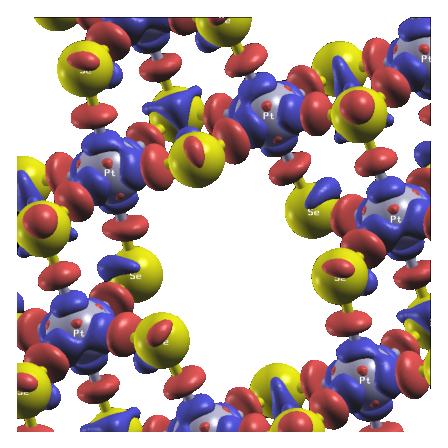
\epsfig{file=figRes/PtSe2/def/ptse2_carga, scale=0.9}
		\label{Sim:fig:CargaVacPtse2}
	}
    \subfigure[densidad de spines]{
    	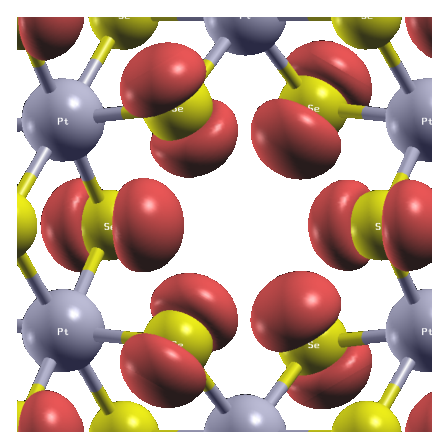
\epsfig{file=figRes/PtSe2/def/ptse2_magz, scale=0.9}
    	\label{Sim:fig:MagzVacPtse2}
    }
  \caption[Iso superficies de la densidad de carga y de spin en el PtSe\textsubscript{2} con vacancia de Platino.]{Isosuperficies de la densidad de carga (\ref{Sim:fig:CargaVacPtse2}) y la densidad de spines (\ref{Sim:fig:MagzVacPtse2} del PtSe\textsubscript{2} con un valor de $0.001 e/\AA^3$. }
\end{figure}


 En el caso del PtS\textsubscript{2}  se observa en la figura \ref{Sim:fig:CargaVacPts2}  la densidad de carga  cerca de la vacancia y es posible observar los enlaces covalentes entre los \'atomos de Platino y Azufre y en la regi\'on de la vacancia se observa que los orbitales $p_z$ y el $p_y$ se hibridizan tal como sucede con el  ptSe\textsubscript{2}. En cuanto la magnetizaci\'on se    tiene que la densidad de spines se concentra en los \'atomos cercanos a la vacancia, debido a que los electrones no se encuentran formando enlaces y se puede notar que dicha distribuci\'on es la esperada en acuerdo a la densidad parcial de estados para el azufre (fig. \ref{Sim:fig:pdosSvacpts2}).
 \begin{figure}[!hbt]
 	\centering
 	\subfigure[densidad de carga]{
 		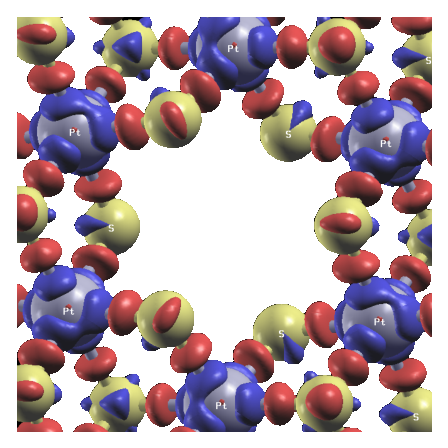
\epsfig{file=figRes/PtS2/def/densidades/pts2_carga, scale=0.9}
 		\label{Sim:fig:CargaVacPts2}
 	}
 	\subfigure[densidad de spines]{
 		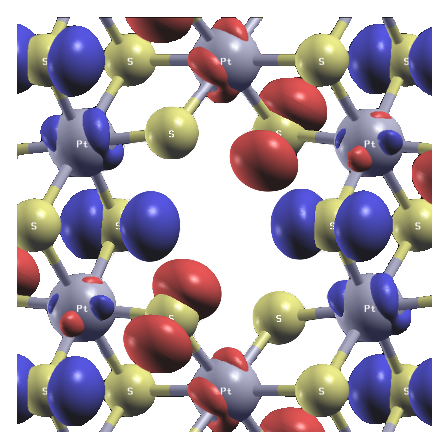
\epsfig{file=figRes/PtS2/def/densidades/pts2_magz, scale=0.9}
 		\label{Sim:fig:MagzVacPts2}
 	}
 	\caption[Iso superficies de la densidad de carga y de spin en el PtS\textsubscript{2} con vacancia de Platino.]{Isosuperficies de la densidad de carga (\ref{Sim:fig:CargaVacPts2}) y la densidad de spines (\ref{Sim:fig:MagzVacPts2} del PtS\textsubscript{2} con un valor de $0.001 e/\AA^3$. }
 \end{figure}     
\subsection{Vacancia de Vanadio en VSe\textsubscript{2} y VS\textsubscript{2}} \label{Sim:subsec:vacV}
Es importante analizar esta clase de defectos debido a que se observa un fen\'omeno distinto a los materiales con Platino, ya que en lugar de que los \'atomos de Selenio y Azufre, se alejen entre  si estos se acercan. En la figura \ref{Sim:fig:vacV} se detallan las superceldas con la vacancia de Vanadio con las posiciones de los \'atomos ya optimizadas.
\newline
\begin{figure}[!hbt]
	\centering
	\subfigure[VSe\textsubscript{2}]{
		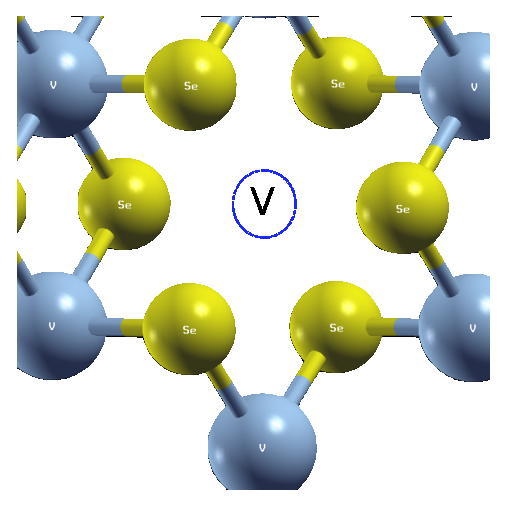
\epsfig{file=figRes/VSe2/def/vacVse2_def, scale=0.7}
		\label{Sim:fig:vacVvse2}
	}
    \subfigure[VS\textsubscript{2}]{
    	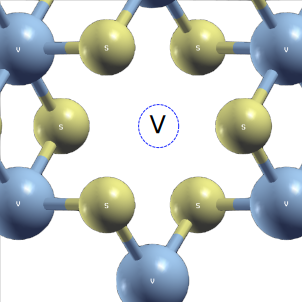
\epsfig{file=figRes/VS2/def/vs2_def, scale=0.7}
    	\label{Sim:fig:vacVvs2}
    }
  \caption[Superceldas de VSe\textsubscript{2} y VS\textsubscript{2} con vacancia de vanadio.]{Superceldas con la vacancia de Vanadio. Visualizada con XcrySDen.}
  \label{Sim:fig:vacV}
\end{figure}

En la figura \ref{Sim:fig:cargavacV} se muestra la distribuci\'on de carga en la regi\'on de la vacancia en el VSe\textsubscript{2} y VS\textsubscript{2}, en donde se puede observar que no existe distribuci\'on de carga en la posici\'on en donde se ubicaba el \'atomo de Vanadio, lo cual explica el motivo por el cual no se separan los \'atomos  vecinos de la vacancia tal como sucede con el PtSe\textsubscript{2} y PtS\textsubscript{2}.
\newline
\begin{figure}[!hbt]
	\centering
	\subfigure[VSe\textsubscript{2}]{
		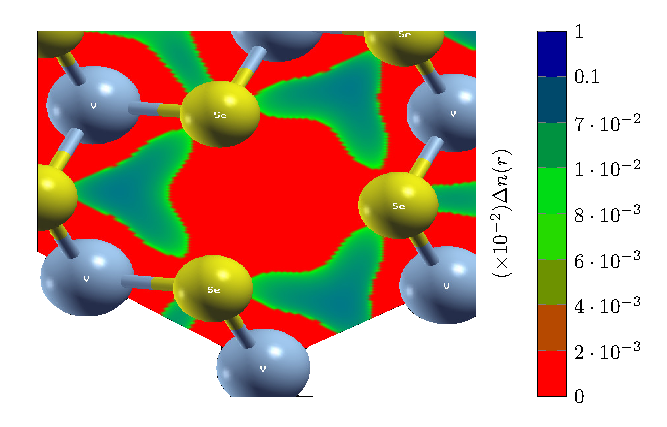
\epsfig{file=figRes/VSe2/def/densidad/densPos/densidadpos, scale=0.9}
		\label{Sim:fig:cargavacVSe2}
	}
	\subfigure[VS\textsubscript{2}]{
		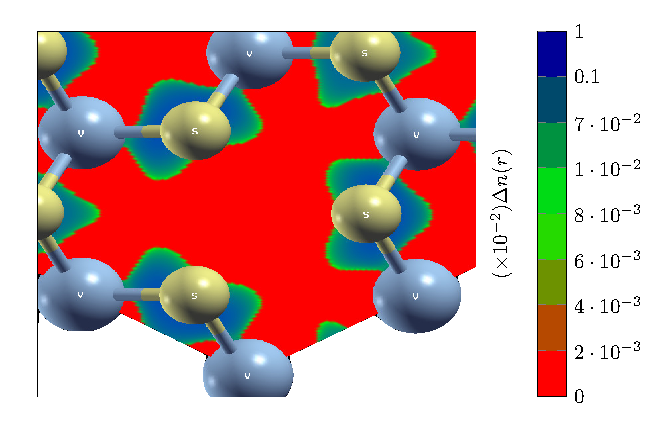
\epsfig{file=figRes/VS2/def/dens/densPos/densidadpos, scale=0.9}
		\label{Sim:fig:cargavacVS2}
	}
\caption[Densidad de carga en el VSe\textsubscript{2} yVS\textsubscript{2}]{densidad de carga en la regi\'on de la vacancia en el VSe\textsubscript{2} y VS\textsubscript{2} visualizada con XcrySDen }
\label{Sim:fig:cargavacV}	
\end{figure}
%\newline
\begin{figure}[!hbt]
	\centering
	\includegraphics[scale=1]{figRes/VSe2/def/bandas/soc/bandasDOS.pdf}
	\caption[Diagrama de bandas y densidad de estados con el efecto spin-\'orbita del VSe\textsubscript{2} con vacancia de Vanadio.]{Estructura de bandas y densidad de estados de la supercelda de Vse\textsubscript{2} con un vacancia de vanadio y el efecto de spin-\'orbita.}
	\label{Sim:fig:vacVvse2band}
\end{figure}
%\newline
\par En la figura \ref{Sim:fig:vacVvse2band} se muestra el diagrama de bandas y la densidad de estados  del  VSe\textsubscript{2}. En cuanto a la densidad de estados se observa que mantiene  una forma muy similar al caso de la estructura sin defectos (fig. \ref{Sim:fig:bandSocVSe2}). En cuanto al diagrama de bandas  se observan mas bandas que en el caso que se estudi\'o en la sub secci\'on \ref{Sim:subsec:vse2cU} y esto es debido a que las estructuras tienen mas \'atomos que en el caso de la celda unitaria y no necesariamente se deben a la vacancia, en la figura \ref{Sim:fig:bandasvse2orb} se observa la distribuci\'on de los orbitales en el espacio rec\'iproco y se puede notar que los orbitales $p$ del \'atomo de selenio vecino ala vacancia se encuentran localizados en ciertas posiciones cercanas al nivel de Fermi. 
\begin{figure}[!hbt] 
	\centering
	\includegraphics[scale=1]{figRes/VSe2/def/bandas/soc/bandasSe.pdf}
	\caption[Distribuci\'on de los orbitales de los \'atomos en el diagrama de bandas del VSe\textsubscript{2} con vacancia de Vanadio.]{Distribuci\'on de los orbitales $p$ del \'atomo de Selenio y $d$ del Vanadio.}
	\label{Sim:fig:bandasvse2orb}
\end{figure}
\newline
\par En la figura \ref{Sim:fig:VSe2noSOCcavband} se muestra el diagrama de bandas indicando a qu\'e spin pertenecen, not\'andose ahora la diferencia de poblaci\'on entre los electrones de spin $\uparrow$ y $\downarrow$ provocando una magnetizaci\'on de $0.48 ~\mu_{B}/ celda$. Si se compara la magnetizaci\'on de la supercelda sin defectos que es $3.19~\mu_{B}/celda$, se nota que se reduce la magnetizaci\'on considerablemente y para poder explicar la raz\'on de este fen\'omeno, es necesario observar los cambios en las contribuciones de los \'atomos del sistema a la magnetizaci\'on total. 
\begin{figure}[!hbt]
	\centering
	\includegraphics[width=13cm, height=9cm]{figRes/VSe2/def/bandas/nosoc/bandasDOSnoSoc.pdf}
	\caption[Diagrama de bandas y densidad de estados del VSe\textsubscript{2} con vacancia de Vanadio.]{Diagrama de bandas y la densidad de estados para los spin $\uparrow$ y $\downarrow$ mostrando la distribuci\'on de estos} 
	\label{Sim:fig:VSe2noSOCcavband}
\end{figure}
%\newline
\par Analizando el comportamiento de los \'atomos de Selenio que no es vecino de la vacancia, se observa que  no se ve afectado directamente por la vacancia, ya que presenta una magnetizaci\'on de $-0.012~\mu_{B}$, la cual es menor que en el caso expuesto en la subsecci\'on \ref{Sim:subsec:vse2cU}. En la figura \ref{Sim:fig:pdosSeVse2} se observa la densidad de estados de los orbitales $p$ del \'atomo de Selenio con sus enlaces completos y es posible apreciar que la mayor\'ia de los estados provienen de los orbitales $p_y$ y $p_z$ y al igual que en el caso sin defectos, existe una regi\'on entre el nivel de Fermi y 0.5 eV por encima de este, en donde no existe una gran contribuci\'on de estados. Para el caso de la densidad de estados del \'atomo vecino  a la vacancia de vanadio (fig. \ref{Sim:fig:pdosSevacVse2}), se puede observar que en la regi\'on pr\'oxima al nivel de Fermi, s\'i existen mas estados que provienen de los orbitales $p_y$ y $p_z$ y, a diferencia de los materiales con Platino, no aumenta la contribuci\'on en la magnetizaci\'on, ya que aportan $-0.007~ \mu_{B}$, por  lo que pr\'acticamente no aportan a la magnetizaci\'on total del sistema. En principio esto no reducir\'ia la magnetizaci\'on del material debido a que en el caso del VSe\textsubscript{2}, la mayor contribuci\'on proviene de los \'atomos de Vanadio.
%\newline
 
\begin{figure}[!hbt]
	\centering
	\includegraphics[scale=1]{figRes/VSe2/def/bandas/nosoc/pdosSe.pdf}
	\caption[Densidad de estados parcial de los orbitales $p$ del \'atomo de Selenio en VSe\textsubscript{2} con vacancia de vanadio]{Densidad de estados parcial de los orbitales $p$ del \'atomo de Selenio con enlaces completos.}
	\label{Sim:fig:pdosSeVse2}
\end{figure}

\begin{figure}[!hbt]
	\centering
	\includegraphics[scale=1]{figRes/VSe2/def/bandas/nosoc/pdosSe_vac.pdf}
	\caption[Densidad de estados parcial de los orbitales $p$ del \'atomo de Selenio vecino a la vacancia en VSe\textsubscript{2} con vacancia de vanadio]{Densidad de estados parcial de los orbitales $p$ del \'atomo de Selenio vecino a la vacancia.}
	\label{Sim:fig:pdosSevacVse2}
\end{figure}
En la figura \ref{Sim:fig:pdosVVse2} se puede  que la distribuci\'on de los orbitales $d_{x^2-y^2}$ y $d_{xy}$ son los que contribuyen mayoritariamente a la densidad de estados en la regi\'on cercana al nivel de Fermi y en los estados de mayor energ\'ia. En la regi\'on mas cercana al n\'ucleo la mayor contribuci\'on proviene de los orbitales $d_{zx}$ y $d_{zy}$; sin embargo, la diferencia de poblaciones proviene principalmente de los orbitales $d_{x^2-y^2}$ y $d_{xy}$ y por lo tanto, los spines siguen teniendo la misma orientaci\'on que en el caso del material sin defectos, pero la magnetizaci\'on se reduce a $0.16~\mu_B$, el cual es un valor 74\% menor al caso del material sin defectos.
\begin{figure}[!hbt]
	\centering
	\includegraphics[scale=1]{figRes/VSe2/def/bandas/nosoc/pdosV.pdf}
	\caption[Densidad de estados parcial de los orbitales $d$ del \'atomo de vanadio en VSe\textsubscript{2} con vacancia de vanadio]{Densidad de estados parcial de los orbitales $d$ del \'atomo de Vanadio.}
	\label{Sim:fig:pdosVVse2}
\end{figure} 
\newline
\begin{figure}[!hbt]
	\centering
	\includegraphics[scale=1]{figRes/VS2/def/bandas/nosoc/bandasSe.pdf}
	\caption[Distribuci\'on de los orbitales de los \'atomos en el diagrama de bandas del VS\textsubscript{2} con vacancia de Vanadio]{Distribuci\'on de los orbitales $p$ y $d$ de Azufre y vanadio en el diagrama de bandas}
	\label{Sim:fig:orbVacVS2bandas}
\end{figure}
\begin{figure}[!hbt]
	\centering
	\includegraphics[scale=1]{figRes/VS2/def/bandas/nosoc/bandasDOSnoSoc.pdf}
	\caption[Diagrama de bandas  y densidad de estados en el VS\textsubscript{2} con vacancia de Vanadio]{Diagrama de bandas y Densidad de Estados del  VS\textsubscript{2}.}
	\label{Sim:fig:VacVS2bandas}
\end{figure}
\par En el caso del VS\textsubscript{2} se tiene un fen\'omeno similar, tal como se observa en la figura \ref{Sim:fig:orbVacVS2bandas} el efecto de la vacancia de Vanadio induce que  ciertas bandas provengan de electrones del \'atomo de azufre cercano a la vacancia y estas se encuentran en posiciones cercanas al nivel de Fermi. dicha distribuci\'on se ve muy similar al del VSe\textsubscript{2}. En la figura \ref{Sim:fig:VacVS2bandas} se muestra el diagrama de bandas correspondiente a a cada spin ($\uparrow,~ \downarrow$) en donde se puede notar que existen bandas bien definidas  para cada spin por debajo del nivel de Fermi y por encima de este, tambi\'en se observa que las bandas para cada spin no son muy distintas. En cuanto a la densidad de estados se puede observar  que las mayores contribuciones provienen del orbital $d$ del Vanadio, aunque la diferencia entre estos y los provenientes del orbital $p$ del Azufre, ya no es tan grande como en el caso del material sin defectos (subsec. \ref{Sim:subsec:VS2}). Adem\'as de que se observa que la diferencia de poblaci\'on entre diferente spin es mas peque\~na que en el caso del material sin deformar, lo cual induce  una magnetizaci\'on de $0.76 ~\mu_B/celda$ y, si se compara con el valor $2.04 ~\mu_B/celda$  que se obtuvo con la supercelda sin defectos, se observa un valor menor. En cuanto el \'atomo de Vanadio en la figura \ref{Sim:fig:pdosVvacVS2} se muestra la densidad de estados parcial de los orbitales $d$ del \'atomo de Vanadio y se observa que la mayor diferencia de poblaci\'on entre los spines $\uparrow$ y $\downarrow$ proviene de los orbitales $d_{zx}$ y $d_{zy}$ en la regi\'on mas cercana al n\'ucleo y de los orbitales $d_{x^2-y^2}$ y $d_{xy}$ en la regi\'on cercana al nivel de Fermi y por lo tanto, la magnetizaci\'on se debe principalmente a la diferencia de poblaci\'on  de estos orbitales y cuyo valor es de $0.215~\mu_{B}$, el cual es un valor menor al que se obtuvo en el material sin defectos.
\begin{figure}[!hbt]
	\centering
	\includegraphics[scale=1]{figRes/VS2/def/bandas/nosoc/pdosV.pdf}
	\caption[Densidad de estados proyectada en los orbitales $d$ del Vanadio en VS\textsubscript{2} con vacancia de Vanadio.]{Densidad de estados parcial de los orbitales $d$ del \'atomo de Vanadio}
	\label{Sim:fig:pdosVvacVS2}
\end{figure}
%\newline
En cuanto  al \'atomo de Azufre, que aun tiene sus tres enlaces, se puede notar en la densidad de estados (fig. \ref{Sim:fig:pdosSVS2}) que la mayor contribuci\'on proviene del orbital $p_x$ en la regi\'on cercana al nivel de Fermi. Es posible notar que la diferencia de la poblaci\'on de spines no es muy grande y por lo tanto, se tiene una magnetizaci\'on de $-0.0092~\mu_B$. Para el \'atomo de azufre cercano a la vacancia se observa en la densidad de estados proyectada (fig. \ref{Sim:fig:pdosSvacVS2}) se puede notar que la mayor contribuci\'on proviene de los orbitales $p_y$ y $p_z$ en la regi\'on cercana al nivel de Fermi. Esto se puede deber a que los orbitales que participaban en los enlaces con el \'atomo de Vanadio se combinan con los orbitales $p_z$;  adem\'as se puede observar que si existen estados por encima del nivel de Fermi, que al igual que en el VSe\textsubscript{2}, se relacionan con estados generados con la vacancia y concuerda con lo observado en la distribuci\'on de los estados de los orbitales en le diagrama de bandas. En cuanto a la diferencia de las poblaciones de spines, esta proviene de estos dos orbitales y se tiene una magnetizaci\'on de   $-0.0038~\mu_{B}$, el cual es un valor peque\~no y se observa el mismo fen\'omeno que en el caso del VSe\textsubscript{2}, en donde la aportaci\'on de los \'atomos calc\'ogenos no contribuyen de la misma manera que en el material sin defectos.
\begin{figure}[!hbt]
	\centering
	\includegraphics[scale=1]{figRes/VS2/def/bandas/nosoc/pdosSe.pdf}
	\caption[Densidad de estados proyectada en los orbitales $p$ del Azufre en VS\textsubscript{2} con vacancia de Vanadio]{Densidad de estados parcial de los orbitales $P$ del \'atomo de Azufre que no se ve afectado por la vacancia de Azufre.}
	\label{Sim:fig:pdosSVS2}
\end{figure}
%\newline

 
\begin{figure}[!hbt]
	\centering
	\includegraphics[scale=1]{figRes/VS2/def/bandas/nosoc/pdosSe_vac.pdf}
	\caption[Densidad de estados proyectada en los orbitales $p$ del Azufre vecino de la vacancia en VS\textsubscript{2} con vacancia de Vanadio]{Densidad de estados parcial de los orbitales $p$ del \'atomo de Azufre vecino de la vacancia.}
	\label{Sim:fig:pdosSvacVS2}
\end{figure}

\par En la figura \ref{Sim:fig:cargaVac} se muestra la densidad de carga del VSe\textsubscript{2} (fig. \ref{Sim:fig:cargaVacVSe2}) y VS\textsubscript{2} (fig. \ref{Sim:fig:cargaVacVS2}), donde  se puede observar que los enlaces entre el calcogenuro y el Vanadio es covalente y que los \'atomos de Azufre y Selenio, que son cercanos a la vacancia de Vanadio, se comportan de la misma manera que los materiales con Platino. Es posible notar que los orbitales $p_z$ y $p_y$ se combinan y se puede notar en la parte inferior de la figura, que el \'atomo que no se ve afectado por la vacancia se conservan sus tres enlaces. 
\begin{figure}[!hbt]
	\centering
	\subfigure[VSe\textsubscript{2}]{
		\epsfig{file=figRes/VSe2/def/densidad/vse2_carga_vac.eps, scale=0.8}
		\label{Sim:fig:cargaVacVSe2}
	}
    \subfigure[VS\textsubscript{2}]{
    	\epsfig{file=figRes/VS2/def/dens/vs2_carga_vac.eps, scale=0.8}
    	\label{Sim:fig:cargaVacVS2}
    	
    }
  \caption[Densidad de electrones en el VSe\textsubscript{2} y VS\textsubscript{2} con vacancia de Vanadio.]{Iso superficies de la densidad de carga con  un valor de $\pm 0.001 e/\AA^3$}
  \label{Sim:fig:cargaVac}
\end{figure}
\newline
En relaci\'on a la densidad de spines (fig. \ref{Sim:fig:magzVacV}) se puede observar que los \'atomos cercanos en la vacancia no aportan una gran cantidad  a la densidad total y lo cual est\'a de acuerdo con lo observado en las densidades de estados de los \'atomos de Azufre y Selenio. 
\begin{figure}[!hbt]
	\centering
	\subfigure[VSe\textsubscript{2}]{
		\epsfig{file=figRes/VSe2/def/densidad/vse2_magz.eps, scale=0.8}
		\label{Sim:fig:magnVacVSe2}
	}
	\subfigure[VS\textsubscript{2}]{
		\epsfig{file=figRes/VS2/def/dens/vs2_magz.eps, scale=0.8}
		\label{Sim:fig:magnVacVS2}
		
	}
\caption[Densidad de spin en el VSe\textsubscript{2} y VS\textsubscript{2} con vacancia de Vanadio.]{Iso superficies de la densidad de spines con  un valor de $\pm 0.0002 e/\AA^3$}
\label{Sim:fig:magzVacV}
\end{figure}
\section{Estudio del efecto de las deformaciones en la magnetizaci\'on} \label{Sim:sec:Str}
\subsection{Efecto en VSe\textsubscript{2} y VS\textsubscript{2}}
Si se aplica una deformaci\'on mec\'anica isotr\'opica descrita en la Figura \ref{Met:fig:strainiso} y cuya magnitud de deformaci\'on se describe por la ecuaci\'on \ref{Met:ec:strain}, se puede observar que la variaci\'on de la magnetizaci\'on en el VSe\textsubscript{2} (fig. \ref{Sim:fig:strVSe2Iso}) y Vs\textsubscript{2} (fig. \ref{Sim:fig:strVS2Iso}) presentan  un comportamiento casi lineal con respecto a la variaci\'on de la deformaci\'on con  un valor que va desde $-0.05$ a $+0.05$; para el  VSe\textsubscript{2} la magnetizaci\'on cambia de $0.3$ a $1.04 ~\mu_B/celda$,  indicando un cambio en la magnetizaci\'on de $0.74~\mu_{B}/celda$. En el caso del VS\textsubscript{2} la variaci\'on de la magnetizaci\'on es de $0.23$ a $1 ~ \mu_{B}/celda$, lo cual indica un cambio   de  $0.77~\mu_{B}/celda$, sugiriendo un cambio mayor que en comparaci\'on con el VSe\textsubscript{2}. De igual forma se muestran im\'agenes de las estructuras deformadas con  valores de deformaci\'on  $\varepsilon= -0.05,~0.0,~0.05$. 

\begin{figure}[!hbt]
	\centering
	\subfigure[VSe\textsubscript{2}]{
		\includegraphics[scale=1.1]{figRes/VSe2/str/isotropico/magn.pdf}
		\label{Sim:fig:strVSe2Iso}
	}
    \subfigure[VS\textsubscript{2}]{
    	\includegraphics[scale=1.1]{figRes/VS2/str/isotropico/magn.pdf}
    	\label{Sim:fig:strVS2Iso}
    }
\caption[Magnetizaci\'on del VSe\textsubscript{2} y VS\textsubscript{2} en funci\'on de una deformaci\'on isotr\'opica. ]{Gr\'aficas de la magnetizaci\'on en funci\'on de la deformaci\'on isotr\'opica en VSe\textsubscript{2} y VS\textsubscript{2} mostrando el ajuste lineal de los datos.}
\label{Sim:fig:MgnVx2Iso}
\end{figure}

 Para poder analizar  la variaci\'on de la magnetizaci\'on se consideran los cambios en las distancias entre los distintos \'atomos que est\'an identificadas de acuerdo con lo que se muestra en la figura \ref{Sim:fig:disVX2Iso}. 
 \begin{figure}[!hbt]
 	\centering
 	\epsfig{file=figRes/compIso,scale=0.8}
 	\caption[ Distancias entre \'atomos   VSe\textsubscript{2} y VS\textsubscript{2} utilizados para el estudio de una deformaci\'on isotr\'opica]{Distancias entre \'atomos en el VSe\textsubscript{2} y  VS\textsubscript{2} en donde las esferas grises representran el vanadio y las amarillas El Azufre o Selenio.}
 	\label{Sim:fig:disVX2Iso}
 \end{figure}
\par Si se toma en cuenta el cambio de la distancia entre los dos \'atomos calc\'ogenos, es posible observar que el cambio correspondiente disminuye conforme aumenta la deformación tal y como se aprecia en la figura \ref{Sim:fig:DSVx2Iso} para en Vse\textsubscript{2} y VS\textsubscript{2}. En este caso no se observa  una tendencia parecida a la magnetizaci\'on. En cuanto a la distancia entre el \'atomo de Vanadio y el Azufre  o Selenio, se muestra en la figura \ref{Sim:fig:DVSVx2Iso} la  variaci\'on del cambio de la distancia entre estos dos \'atomos y es posible notar que se comportan de forma lineal y con una tendencia similar a la magnetizaci\'on. En esta figura se muestran adem\'as las lineas de dicha  tendencia y se puede notar que el cambio es mayor en el caso del VS\textsubscript{2}, lo cual  concuerda con lo observado en la magnetización. 

\begin{figure}[!hbt]
	\centering
	\subfigure[VSe\textsubscript{2}]{
		\includegraphics[scale=1]{figRes/VSe2/str/isotropico/dS.pdf}
		\label{Sim:fig:DSVSe2Iso}
	}
	\subfigure[VS\textsubscript{2}]{
		\includegraphics[scale=1]{figRes/VS2/str/isotropico/dS.pdf}
		\label{Sim:fig:DSVS2Iso}
	}
	\caption[Cambio en la distancia entre \'atomos de Selenio o Azufre  y Vanadio en  VSe\textsubscript{2} y VS\textsubscript{2} en funci\'on de una deformaci\'on isotr\'opica]{Cambio en la distancia entre dos \'atomos de Selenio en VSe\textsubscript{2} y Azufre en VS\textsubscript{2}.}
	\label{Sim:fig:DSVx2Iso}
\end{figure}
\begin{figure}[!hbt]
	\centering
	\subfigure[VSe\textsubscript{2}]{
		\includegraphics[scale=1]{figRes/VSe2/str/isotropico/dVS.pdf}
		\label{Sim:fig:DVSVSe2Iso}
	}
	\subfigure[VS\textsubscript{2}]{
		\includegraphics[scale=1]{figRes/VS2/str/isotropico/dVS.pdf}
		\label{Sim:fig:DVSVS2Iso}
	}
	\caption[Cambio en la distancia entre \'atomos de Selenio o Azufre en  VSe\textsubscript{2} y VS\textsubscript{2} en funci\'on de una deformaci\'on isotr\'opica. ]{Cambio en la distancia entre dos \'atomos de Selenio en VSe\textsubscript{2} y Azufre en VS\textsubscript{2}.}
	\label{Sim:fig:DVSVx2Iso}
\end{figure}
\par Para la deformaci\'on anisotr\'opica que se muestra en la figura \ref{Met:fig:strainanis} se observa  en la figura \ref{Sim:fig:MgnVx2Anis} la magnetizaci\'on en funci\'on de la deformaci\'on $\varepsilon_x$  y es posible notar que no existen cambios considerables  de tal forma que se puede argumentar que se mantiene constante; el principal efecto de aplicar dicha deformaci\'on es que ya no existe un \'angulo de $120 \degree$ entre los \'atomos de Vanadio y esto provoca que se pierda la simetr\'ia octaedral; sin embargo, las estructuras no sufren grandes cambios tal y como se puede notar en las figuras \ref{Sim:fig:strVSe2anis} y \ref{Sim:fig:strVS2Anis}.
\begin{figure}[!hbt]
	\centering
	\subfigure[VSe\textsubscript{2}]{
		\includegraphics[scale=1.15]{figRes/VSe2/str/anisotropico/magn.pdf}
		\label{Sim:fig:strVSe2anis}
	}
	\subfigure[VS\textsubscript{2}]{
		\includegraphics[scale=1.15]{figRes/VS2/str/anisotropico/magn.pdf}
		\label{Sim:fig:strVS2Anis}
	}
	\caption[Magnetizaci\'on del VSe\textsubscript{2} y VS\textsubscript{2} bajo una deformaci\'on anisotr\'opica.]{Gr\'aficas de la magnetizaci\'on en funci\'on de la deformaci\'on anisotr\'opica en VSe\textsubscript{2} y VS\textsubscript{2}.}
	\label{Sim:fig:MgnVx2Anis}
\end{figure}
Dicha deformaci\'on provoca que la distancia entre los \'atomos de Azufre o Selenio y Vanadio  sea diferente para cada \'atomo de Vanadio  vecino. En el caso de esta deformaci\'on las dos distancias se siguen comportando de la misma manera y una no, estas dos distancias con comportamientos diferentes se encuentran marcadas por $(S,Se-V)_{1,2}$ en la figura \ref{Sim:fig:disVX2Anis}. De igual forma la distancia entre calc\'ogenos no es la misma y est\'an indicadas por $(S,Se-S,Se)_{1,2}$. 
\begin{figure}[!hbt]
	\centering
	\epsfig{file=figRes/compAnis.eps,scale=0.9}
	\caption[Distancias entre \'atomos   VSe\textsubscript{2} y VS\textsubscript{2} utilizados para el estudio de una deformaci\'on anisotr\'opica.]{Distancias entre \'atomos en el VSe\textsubscript{2} y  VS\textsubscript{2} en la deformaci\'on anisotr\'opica, las esferas grises representan el vanadio y las amarillas El Azufre o Selenio.}
	\label{Sim:fig:disVX2Anis}
\end{figure}
%\newline
Esta 'ultima deformaci\'on se aplic\'o para valores de $\varepsilon_x$ de $-0.03$ a $0.03$, lo que indujo un cambio en el \'angulo entre los \'atomos de Vanadio  de $\pm 3 \degree$ en ambos materiales. Sin embargo no provoca grandes cambios en la distancia entre los \'atomos de vanadio tal y como se observa en la figura \ref{Sim:fig:compdV}  donde se puede notar que el cambio en la deformaci\'on anisotr\'opica es mas peque\~no. Al momento de observar el cambio de las distancias $(S,Se-S,Se)_{1,2}$ que se muestran en la figura \ref{Sim:fig:compdSSVX2}, es posible notar que en el caso del VSe\textsubscript{2}  la variaci\'on de las correspondientes distancias tienen signos contrarios; es decir, que mientras $\Delta (Se-Se)_{1}$  aumenta con el incremento de $\varepsilon_x$,  $\Delta (Se-Se)_{2}$ disminuye. Si se calcula la variaci\'on promedio (que se muestra en la figura \ref{Sim:fig:compdSSeVse2}) se nota que ronda entre $\pm 0.01 \AA$. En el caso del VS\textsubscript{2} (fig. \ref{Sim:fig:compdSSVs2}) los cambios en la variaci\'on de $\Delta (S-S)_{1,2}$  se comportan de la misma manera que en el  VSe\textsubscript{2}. Como se puede notar en  ambos casos el cambio es considerable.
\begin{figure}[!hbt]
	\centering
	\subfigure[VSe\textsubscript{2}]{
		\includegraphics[scale=0.8]{figRes/VSe2/str/com/CompdPt.pdf}
		\label{Sim:fig:compdVVse2}	
	}
	\subfigure[VS\textsubscript{2}]{
		\includegraphics[scale=0.8]{figRes/VS2/str/com/CompdPt.pdf}
	  \label{Sim:fig:compdVVs2}	
	}
	
	\caption[Comparaci\'on del cambio en la distancia entre los \'atomos de Platino por una deformaci\'on isotr\'opica y anisotr\'opica]{Comparaci\'on del cambio en da distancia entre \'atomos de vanadio bajo una deformaci\'on isotr\'opica y otra anisotr\'opica.}
	\label{Sim:fig:compdV}
\end{figure}

\begin{figure}[!hbt]
	\centering
	\subfigure[VSe\textsubscript{2}]{
		\includegraphics[scale=1.1]{figRes/VSe2/str/anisotropico/CompdSS.pdf}
		\label{Sim:fig:compdSSeVse2}	
	}
	\subfigure[VS\textsubscript{2}]{
		\includegraphics[scale=1.1]{figRes/VS2/str/anisotropico/CompdSS.pdf}
		\label{Sim:fig:compdSSVs2}	
	}
 \caption[Variaci\'on de la distancia entre \'atomos de Selenio y Azufre en VSe\textsubscript{2} y VS\textsubscript{2} mediante una deformaci\'on anisotr\'opica]{variaci\'on de las distancias entre \'atomos de Selenio en el VSe\textsubscript{2} y de Azufre en VS\textsubscript{2}.}
 \label{Sim:fig:compdSSVX2}
\end{figure}
%\newline
\par En la figura \ref{Sim:fig:compdSVVX2} se muestra la variaci\'on de la distancia entre el Selenio o Azufre  y el Vanadio, donde se puede observar un comportamiento muy similar al  caso de las distancias entre \'atomos de Azufre o Selenio descritos anteriormente y en la figura \ref{Sim:fig:compdSVVse2} se indica el cambio $\Delta (Se-V)_{1,2}$, en donde se tiene que, es posible observar que  mientras  $\Delta (Se-V)_{1}$ aumenta con el incremento de $\varepsilon_x$, $\Delta (Se-V)_{2}$ disminuye. El cambio promedio de $\Delta (Se-V)$ da un valor que var\'ia entre $-0.004$ y $0.007 ~\AA$.  Para el VS\textsubscript{2} (fig. \ref{Sim:fig:compdSVVs2})
sucede el mismo comportamiento  en donde es posible observar un cambio promedio que se encuentra entre el mismo rango que en el VSe\textsubscript{2}.
\begin{figure}[!hbt]
	\centering
	\subfigure[VSe\textsubscript{2}]{
		\includegraphics[scale=1]{figRes/VSe2/str/anisotropico/CompdVS.pdf}
		\label{Sim:fig:compdSVVse2}	
	}
	\subfigure[VS\textsubscript{2}]{
		\includegraphics[scale=1]{figRes/VS2/str/anisotropico/CompdVS.pdf}
		\label{Sim:fig:compdSVVs2}	
	}
	\caption[Variaci\'on de la distancia entre los \'atomos calc\'ogenos y el \'atomo de vanadio  (VSe\textsubscript{2} y VS\textsubscript{2})bajo una deformaci\'on anisotr\'opica]{variaci\'on de las distancias entre \'atomos de Selenio en el VSe\textsubscript{2} y de Azufre en VS\textsubscript{2}.}
	\label{Sim:fig:compdSVVX2}
\end{figure}
%\newline
\par Dado que el cambio en la distancia entre los \'atomos de Selenio o Azufre  y el \'atomo de Vanadio es muy peque\~no, entonces la interacci\'on entre estos dos \'atomos no var\'ia considerablemente causando que la magnetizaci\'on individual de estos \'atomos pr\'acticamente no cambia tal y como se muestra en la figura \ref{Sim:fig:cmagVX2}. 
\begin{figure}[!hbt]
	\centering
	\subfigure[VSe\textsubscript{2}]{
		\includegraphics[scale=1.1]{figRes/VSe2/str/anisotropico/CompMag.pdf}
		\label{Sim:fig:cmagVse2}	
	}
	\subfigure[VS\textsubscript{2}]{
		\includegraphics[scale=1.1]{figRes/VS2/str/anisotropico/CompMag.pdf}
		\label{Sim:fig:cmagVs2}	
	}
	\caption[Magnetizaci\'on de los \'atomos individuales en el VS\textsubscript{2} y VSe\textsubscript{2} bajo una deformaci\'on anisotr\'opica]{Magnetizaci\'on del \'atomo de vanadio y selenio o Azufre en el VSe\textsubscript{2} (\ref{Sim:fig:cmagVse2}) y VS\textsubscript{2} (\ref{Sim:fig:cmagVs2}) bajo una deformaci\'on anisotr\'opica.}
	\label{Sim:fig:cmagVX2}
\end{figure}
%\newline
\par En el caso de la deformaci\'on isotr\'opica se observa un fen\'omeno diferente: en la figura \ref{Sim:fig:cmagVX2I} es posible notar que la magnetizaci\'on del \'atomo de Vanadio se comporta de la misma manera que la magnetizaci\'on de todo el sistema (fig. \ref{Sim:fig:MgnVx2Iso}) y en ambos caso se observa un comportamiento muy similar de la magnetizaci\'on del \'atomo de Vanadio para  VSe\textsubscript{2} y  VS\textsubscript{2}. Para el caso de los \'atomos de Azufre y Selenio se encuentra que el valor negativo aumenta tendiendo  a $-0.092 ~\mu_{B}$ para el selenio y $-0.07~\mu_B $ para el Azufre. 
\begin{figure}[!hbt]
	\centering
	\subfigure[VSe\textsubscript{2}]{
		\includegraphics[scale=1.1]{figRes/VSe2/str/isotropico/CompMag.pdf}
		\label{Sim:fig:cmagVse2I}	
	}
	\subfigure[VS\textsubscript{2}]{
		\includegraphics[scale=1.1]{figRes/VS2/str/isotropico/CompMag.pdf}
		\label{Sim:fig:cmagVs2I}	
	}
	\caption[Magnetizaci\'on de los \'atomos individuales en el VS\textsubscript{2} y VSe\textsubscript{2} bajo una deformaci\'on isotr\'opica]{Magnetizaci\'on del \'atomo de vanadio y selenio o Azufre en el VSe\textsubscript{2} (\ref{Sim:fig:cmagVse2I}) y VS\textsubscript{2} (\ref{Sim:fig:cmagVs2I}) bajo una deformaci\'on isotr\'opica.}
	\label{Sim:fig:cmagVX2I}
\end{figure} 
\subsection{Efecto de una vacancia de Platino en PtSe\textsubscript{2} y PtS\textsubscript{2}} \label{Sim:subsec:strPtx2}
\begin{figure}[!hbt]
	\centering
	\subfigure[PtSe\textsubscript{2}]{
		\includegraphics[scale=1.1]{figRes/PtSe2/str/isotropico/magn.pdf}
		\label{Sim:fig:magnPtSe2}
	}
	\subfigure[PtS\textsubscript{2}]{
		\includegraphics[scale=1.1]{figRes/PtS2/str/isotropico/magn.pdf}
		\label{Sim:fig:magnPtS2}
		
	}
	\caption[Magnetizaci\'on del PtSe\textsubscript{2} y PtSe\textsubscript{2} con una vacancia de Platino bajo una deformaci\'on isotr\'opica]{Magnetizaci\'on en funci\'on de una deformaci\'on isotr\'opica en PtSe\textsubscript{2} y PtS\textsubscript{2} con una vacancia de Platino}
	\label{Sim:fig:magnPtX2}
\end{figure}
En cuanto el estudio del PtSe\textsubscript{2} y el PtS\textsubscript{2} se puede apreciar en la figura \ref{Sim:fig:magnPtX2} que muestra muestra una deformaci\'on isotr\'opica en donde $\varepsilon$ toma valores entre $\pm 0.05$ y es posible notar que a cierto valor de $\varepsilon$ la magnetizaci\'on correspondiente se desvanece, $\varepsilon_{m0}=0.04$ para el PtSe\textsubscript{2} y $\varepsilon_{m0}=0.05$ para el  PtS\textsubscript{2}. Es posible tambi\'en notar que existe una regi\'on en la que la magnetizaci\'on aumenta antes de reducirse a cero y en el PtSe\textsubscript{2} se observa una reducci\'on en la
magnetizaci\'on para valores negativos de $\varepsilon$. Tambi\'en se muestran las im\'agenes de las estructuras deformadas que corresponden a valores de $\varepsilon$ en donde la magnetizaci\'on es cero o mucho menor al valor a $\varepsilon=0$. Posteriormente se analizan el cambio de las distancias entre los \'atomos que se observan en la figura \ref{Sim:fig:defIsoPtX2}.
\begin{figure}[htbp]
	\centering
	\epsfig{file=figRes/compIsoDef, scale=0.4}
	\caption[Estudio de distancias en sistemas con Platino y una vacancia bajo una deformaci\'on isotr\'opica]{Distancias entre \'atomos que se utilizan para estudiar una desinformación isotrópica, las esferas grises representan los \'atomos de Platino y las amarillas a \'atomos de Selenio o  azufre. }
	\label{Sim:fig:defIsoPtX2}
\end{figure}
\par Ahora se estudian los  cambios de $(S,Se-S,Se)_{1,2}$. En la figura \ref{Sim:fig:compdSePPtX2} se muestra el cambio $\Delta (S,Se-S,Se)_{1,2}$ en PtSe\textsubscript{2} y PtS\textsubscript{2}. Hay que hacer notar que los cambios se calcularon con respecto a la estructura sin defectos.  En el caso del PtSe\textsubscript{2} (fig. \ref{Sim:fig:compdSePPtSe2}) es posible observar que $\Delta (Se-Se)_{1}$ se mantiene constante hasta que se adquiere un valor de la deformaci\'on de $\varepsilon=0.04$ en donde toma un valor negativo, indicando que los \'atomos de acercan. En el caso del PtS\textsubscript{2} (fig. \ref{Sim:fig:compdSePPtS2}) sucede el mismo fen\'omeno, pero el cambio de  la distancia $\Delta (S-S)_{1}$ no sucede súbitamente como en el PtSe\textsubscript{2} sino que es gradual hasta que se adquiere un valor negativo para $\varepsilon=0.05$. Para  el   $\Delta (S,Se-S,Se)_{2}$  se observa que el valor aumenta gradualmente hasta que el valor  $\Delta (S,Se-S,Se)_{1}$ se vuelve negativo y en ese momento $\Delta (S,Se-S,Se)_{2}$ tambi\'en se reduce. Para el  PtS\textsubscript{2} tambi\'en se observa aun cambio gradual tal y como se puede ver  en $\Delta (S-S)_{1}$ y la raz\'on por la cual  se reduce la magnetización es debido a que se   forman enlaces entre los \'atomos de Azufre  o Selenio son vecinos a la vacancia.
\begin{figure}[!hbt]
	\centering
	\subfigure[PtSe\textsubscript{2}]{
		\includegraphics[scale=0.9]{figRes/PtSe2/str/isotropico/CompdS.pdf}
		\label{Sim:fig:compdSePPtSe2}
	}
	\subfigure[PtS\textsubscript{2}]{
		\includegraphics[scale=0.9]{figRes/PtS2/str/isotropico/CompdS.pdf}
		\label{Sim:fig:compdSePPtS2}
	}
	\caption[Cambio en las distancias de Selenio o Azufre en PtSe\textsubscript{2} yPtS\textsubscript{2} con una vacancia de Platino bajo una deformaci\'on isotr\'opica]{Comparaci\'on del cambio entre \'atomos de Selenio en el PtSe\textsubscript{2} (\ref{Sim:fig:compdSePPtSe2}) y de Azufre en PtS\textsubscript{2} (\ref{Sim:fig:compdSePPtS2}.)
	}
	\label{Sim:fig:compdSePPtX2}
\end{figure}
\begin{figure}[!hbt]
	\centering
	\subfigure[PtSe\textsubscript{2}]{
		\includegraphics[scale=1.1]{figRes/PtSe2/str/anisotropico/magn.pdf}
		\label{Sim:fig:magnPtSe2anis}
	}
	\subfigure[PtS\textsubscript{2}]{
		\includegraphics[scale=1.1]{figRes/PtS2/str/anisotropico/magn.pdf}
		\label{Sim:fig:magnPtS2anis}
		
	}
	\caption[Magnetizaci\'on del PtSe\textsubscript{2} y PtSe\textsubscript{2} con una vacancia de Platino bajo una deformaci\'on anisotr\'opica]{Magnetizaci\'on en funci\'on de una deformaci\'on anisotr\'opica en PtSe\textsubscript{2} y PtS\textsubscript{2} con una vacancia de Platino}
	\label{Sim:fig:magnPtX2anis}
	
\end{figure}
\par En relaci\'on a la deformaci\'on anisotr\'opica se puede observar en la figura \ref{Sim:fig:magnPtX2anis} la magnetizaci\'on en  funci\'on de  $\varepsilon_x$. En el caso de PtSe\textsubscript{2} $\varepsilon_x$ toma valores de $-0.05$ a $0.03$. De $-0.03$ a $0.01$, la magnetizaci\'on es diferente de cero y se mantiene constante con un valor de $2.55 ~\mu_{B}/celda$ y  en la figura \ref{Sim:fig:magnPtSe2anis} las im\'agenes de las estructuras son mostradas al aplicar una deformaci\'on $\varepsilon$ de $-0.04$ y $0.02$ que corresponde a la desaparici\'on de la magnetizaci\'on, se puede notar que las estructuras ya no tienen la simetr\'ia octaedral, donde la forma se asemeja a un rect\'angulo en la regi\'on de vacancia y esto es de  esperarse debido a que se comprime en la direcci\'on $x$ y se expande en $y$ y viceversa. Para el PtSe\textsubscript{2} no fue posible observar una disminuci\'on de la magnetizaci\'on en valores negativos de $\varepsilon_x$ que se mantiene casi constante con un valor de $2.6 ~\mu_{B}/celda$ hasta que se alcanza un valor de $\varepsilon_x=0.04$ la magnetizaci\'on desaparece. En la figura \ref{Sim:fig:magnPtS2anis} se presenta la imagen de la estructura cuando se aplica la deformaci\'on $\varepsilon_x=0.04$ observ\'andose un comportamiento de la misma manera que en el caso del PtSe\textsubscript{2}. Para poder analizar los cambios estructurales bajo esta deformaci\'on anisotr\'opica se estudian las variaciones de las distancias por la aplicaci\'on de una deformaci\'on $\varepsilon_y =-\varepsilon_y$ con respecto al caso en el que no existe la vacancia en el sistema. En la figura \ref{Sim:fig:defAnisPtX2} se presentan dichas distancias y como es de notar esta deformaci\'on induce m\'as cambios en las distancias debido a que no se est\'a aplicando en los ejes del material. 
\begin{figure}[!hbt]
	\centering
	\includegraphics[scale=0.3]{figRes/compAnisDef.eps}
	\caption[Estudio de distancias en sistemas con Platino y una vacancia bajo una deformaci\'on anisotr\'opica]{Distancias entre \'atomos que se utilizan para estudiar una desinformación anisotr\'opica, las esferas grises representan los \'atomos de Platino y las amarillas a \'atomos de Selenio o  azufre. }
	\label{Sim:fig:defAnisPtX2}
\end{figure}
\begin{figure}[!hbt]
	\centering
	\subfigure[PtSe\textsubscript{2}]{
		\includegraphics[scale=1]{figRes/PtSe2/str/anisotropico/CompdS.pdf}
		\label{Sim:fig:compdSePPtSe2A}
	}
	\subfigure[PtS\textsubscript{2}]{
		\includegraphics[scale=1]{figRes/PtS2/str/anisotropico/CompdS.pdf}
		\label{Sim:fig:compdSePPtS2A}
	}
	\caption[Cambio en las distancias de Selenio o Azufre en PtSe\textsubscript{2} yPtS\textsubscript{2} con una vacancia de Platino bajo una deformaci\'on anisotr\'opica]{Comparaci\'on del cambio entre \'atomos de Selenio en el PtSe\textsubscript{2} (\ref{Sim:fig:compdSePPtSe2A}) y de Azufre en PtS\textsubscript{2} (\ref{Sim:fig:compdSePPtS2A} )en una deformaci\'on anisotr\'opica.
	}
	\label{Sim:fig:compdSePPtX2A}
\end{figure}
\par En la figura \ref{Sim:fig:compdSePPtX2A} se muestran los cambios de las distancias entre los \'atomos de Selenio en el Ptse\textsubscript{2} (fig. \ref{Sim:fig:compdSePPtSe2A}) y de Azufre en PtS\textsubscript{2} \ref{Sim:fig:compdSePPtS2A}). El comportamiento es diferente en los dos materiales: para el PtSe\textsubscript{2} se observa que para valores a partir de  $\varepsilon_x = -0.04 $,  $\Delta (Se-Se)_1$ adquiere valores negativos y \'esta es la principal raz\'on por la que la magnetizaci\'on desaparece; posteriormente conforme se aumenta la deformación $\varepsilon_x$,  el cambio en $\Delta (Se-Se)_1$ aumenta mientras que $\Delta (Se-Se)_2$ disminuye. Dicho comportamiento tambi\'en se observa en el PtS\textsubscript{2},en donde cuando se llega a un valor de $\varepsilon_x= 0.02$ para el PtSe\textsubscript{2} y $\varepsilon_x= 0.04$. En el caso del PtS\textsubscript{2}, $\Delta (S,Se-S,Se)_2$ toma un valor negativo y $\Delta (S,Se-S,Se)_1$ crece hasta aproximarse a $1~\AA$. Dichos cambios ser\'ian los causantes de formar la estructuras que se muestran en la figura \ref{Sim:fig:magnPtX2anis}. En cuanto a $\Delta (S,Se-S,Se)_3$, en ambos materiales se observa un comportamiento similar con $\Delta (S,Se-S,Se)_2$.
\begin{figure}[!hbt]
	\centering
	\subfigure[PtSe\textsubscript{2}]{
		\includegraphics[scale=0.9]{figRes/PtSe2/str/isotropico/CompMagn.pdf}
		\label{Sim:fig:magnCptse2iso}
	}
	\subfigure[PtS\textsubscript{2}]{
		\includegraphics[scale=0.9]{figRes/PtS2/str/isotropico/CompMagn.pdf}
		\label{Sim:fig:magnCpts2iso}
	}
	\caption{Magnetizaci\'on correspondiente a cada \'atomo de PtSe\textsubscript{2} yPtS\textsubscript{2} sujetos a una deformaci\'on isotr\'opica}
	\label{Sim:fig:magnCptx2iso}
\end{figure}
\par En la figura \ref{Sim:fig:magnCptx2iso} se muestra la magnetizaci\'on de los respectivos elementos en PtSe\textsubscript{2} y  PtS\textsubscript{2}, en donde es posible notar en la figura \ref{Sim:fig:magnCptse2iso} que para el caso del PtSe\textsubscript{2} se observa que la mayor contribución proviene de los átomos de Selenio cercanos a la vacancia. Dicha magnetización se mantiene constante con el valor para la magnetización descrito en la sub sección \ref{Sim:subsec:vacPt}. Para  los otros \'atomos se obtienen magnetizaciones con los valores descritos en dicha sub secci\'on,  pero cuando la magnetizaci\'on del \'atomo de Selenio se reduce a cero estos tambi\'en lo hacen. Es posible notar que la magnetizaci\'on  desaparece cuando $\Delta (Se-Se)_{1}$ se vuelve negativo indicando que los \'atomos de Selenio de diferente capa se acercan mas de lo que estaban antes de introducir la vacancia. En el caso de una deformaci\'on anisotr\'opica se muestra la magnetizaci\'on de los \'atomos de Selenio vecino de la vacancia y otro que no lo es y  el Platino, en la figura \ref{Sim:fig:magnCptx2aniso} es posible notar que bajo esta deformaci\'on se reduce el valor de la deformaci\'on $\varepsilon_x$ en la cual se induce a cero la magnetizaci\'on.  Al igual que en la deformaci\'on isotr\'opica, cuando la distancia entre \'atomos de Selenio se vuelve negativa, la magnetizaci\'on se reduce a cero y esto se puede notar para $\Delta (Se-Se)_1$ para valores de $\varepsilon_x$ negativos y $\Delta (Se-Se)_2$ para valores de $\varepsilon_x$ positivos, tal y como se observa en la figura \ref{Sim:fig:compdSePPtSe2A}. En el caso del PtS\textsubscript{2} para la deformación isotrópica, se puede observar en la figura \ref{Sim:fig:magnCpts2iso} un comportamiento similar que para el PtSe\textsubscript{2} con la diferencia de que en este caso la magnetización no se reduce para valores de $\varepsilon_x$ negativos y el aumento de la magnetizaci\'on que se observa en la figura \ref{Sim:fig:magnPtS2},  se puede notar que proviene  principalmente del \'atomo de Platino  y cuando $\Delta (S-S)_1$ toma valores negativos. La magnetizaci\'on de cada elemento se reduce a cero. Para una deformaci\'on anisotr\'opica (fig. \ref{Sim:fig:magnCpts2aniso}),  para valores negativos de $\varepsilon_x$ no se observa la reducci\'on a cero de la magnetizaci\'on, lo cual concuerda con lo observado en la figura \ref{Sim:fig:compdSePPtS2A}, en donde no existen valores negativos para $\Delta (S-S)_{1,2}$, y cuando  $\varepsilon_x=0.04$ la magnetización se desaparece y en la figura \ref{Sim:fig:compdSePPtS2A} se puede notar que $\Delta (S-S)_2$ se vuelve negativo.

%\newline
\begin{figure}[!hbt]
	\centering
	\subfigure[PtSe\textsubscript{2}]{
		\includegraphics[scale=0.85]{figRes/PtSe2/str/anisotropico/CompMagn.pdf}
		\label{Sim:fig:magnCptse2aniso}
	}
	\subfigure[PtS\textsubscript{2}]{
		\includegraphics[scale=0.85]{figRes/PtS2/str/anisotropico/CompMagn.pdf}
		\label{Sim:fig:magnCpts2aniso}
	}
	\caption{Magnetizaci\'on correspondiente a cada \'atomo de PtSe\textsubscript{2} yPtS\textsubscript{2} de una deformaci\'on anisotr\'opica}
	\label{Sim:fig:magnCptx2aniso}
\end{figure}
\endinput
